\chapter{Appendix - Chapter 2}
\label{ch:appendix_ch2}

\section{Microbiology: additional information}
\subsection{DNA extraction protocol}
The protocol used for DNA extraction was adapted from the Lysis Protocol I detailed by \citep{lever2015modular}.
Initially, filters were added to \SI{5}{\milli\litre} bead-beating tubes, which were then filled to \SIrange{10}{20}{\percent} of their volume with \SI{0.1}{\milli\metre} Zirconium beads.
Next, \SI{1.5}{\milli\litre} of lysis solution I was added, followed by vigorous homogenization through inverting and tapping.
This was then combined with \SI{3}{\milli\litre} of cold phenol-chloroform-isoamyl alcohol (25:24:1) and vortexed briefly.
The mixture underwent bead-beating for two 30-second intervals at 5000 shakes, with a one-minute pause in between.
This allowed for complete dissolution of the PES-filter.
Subsequently, the sediment was spun down at \SI{10000}{\times $g$} and \SI{4}{\celsius} for \SI{10}{\minute}, and the supernatant was transferred to a clean Eppendorf tube.
To this, one volume of cold 24:1 chloroform-isoamyl alcohol was added, mixed by vortexing for \SI{10}{\second}, and then centrifuged at the same conditions.
This washing step was repeated once, ensuring careful transfer to avoid chloroform and particle inclusion.
DNA was precipitated by adding LPA to a concentration of \SI{20}{\micro\gram\per\milli\litre} and 0.1 volumes of \SI{5}{\molar} sodium chloride to each extract, followed by one volume of isopropanol.
After thorough mixing, the samples were precipitated at \SI{-20}{\celsius} for \SI{2}{\hour}.
The DNA was then centrifuged at room temperature at \SI{10000}{\times $g$} for \SI{20}{\minute}, the supernatant discarded, and the pellet washed twice with \SI{800}{\micro\litre} of \SI{70}{\percent} ethanol, with centrifugation for \SI{10}{\minute} between washes.
The dried pellet was then re-suspended in molecular-grade water by adding water, letting it stand for \SI{5}{\minute} on ice, and gently shaking if necessary until fully dissolved.

\subsection{Quantitative polymerase chain reaction (qPCR)}
The abundance of archaeal \citep{cadillo2006vertical, yu2018growth} and bacterial \citep{lever2015modular, ohkuma1998phylogenetic} 16S rRNA, \textit{mcrA} \citep{steinberg2009mcra}, eukaryotic 18S rRNA \citep{torti2015extraction, hardy2010carbon}, and ammonia-oxidizing Archaea \citep{francis2005ubiquity} and Bacteria \citep{rotthauwe1997ammonia} was quantified using a Light Cycler II (Roche Molecular Systems, Inc.) and the SYBR-Green assay as outlined by Lever et al. \citep{lever2015modular}.
The reaction mixture for the SYBR-Green assay consisted of five parts of 2xSYBR Green I Master (Roche), one part bovine serum albumin (BSA, \SI{10}{\milli\gram\per\milli\litre}, New England Biolabs), 0.5 parts each of forward and reverse primers (\SI{10}{\micro\molar}), and one part molecular-grade water.
Reactions were configured by combining \SI{8}{\micro\litre} of the master mix with \SI{2}{\micro\litre} of DNA template, totaling a \SI{10}{\micro\litre} reaction volume.
Detailed parameters for each run can be found in the corresponding Excel files (xlsx) linked in the Supplementary Appendix.

\subsection{Library preparation}
The initial phase of library preparation involved a boost PCR to standardize concentrations across all samples.
The number of PCR cycles was set based on the threshold cycle (Ct) number obtained from bacterial and archaeal quantitative PCR (qPCR), with an addition of three cycles to ensure uniform template amounts.
Both extraction blanks and PCR negative controls were amplified concurrently to monitor for any contamination.
Subsequent amplification included a tail PCR of 10 cycles to enhance amplicon diversity, followed by an index PCR of 8 cycles for sequencing adapter addition.
Amplicons from the tail and index PCR steps were purified using the Agencourt AMPure XP system (Beckman Coulter) at a ratio of 0.8:1.
The integrity and size of the purified products were verified on an agarose gel using the Bio-Rad Gel Doc 2000 system.
Quantitative assessment of the indexed products was performed on a Spark 10M Multimode Microplate Reader (Tecan) to determine precise concentrations for equimolar pooling.
The pooled library was then evaluated for size distribution and DNA concentration using a 2200 TapeStation with a High Sensitivity D1000 ScreenTape assay (Agilent Technologies) and quantified with a Qubit 2.0 Fluorometer using the Qubit dsDNA BR Assay Kit (Thermo Fisher Scientific).
Finally, the prepared amplicon pool was loaded onto a MiSeq Personal Sequencer (Illumina), utilizing the 600PE kit, at the Genomic Diversity Centre (GDC) Zurich.
A \SI{10}{\percent} PhiX spike was included to ensure sequencing quality and reliability.

\subsection{Bioinformatics}
Initially, sequences underwent a quality assessment using FastQC \citep{andrews2010fastqc}, followed by the removal of residual PhiX sequences and low-complexity reads using usearch \citep{edgar2016unoise2}.
Subsequent steps involved trimming of reads and assembly into amplicons via usearch.
We implemented a stringent quality filtering step with prinseq-lite to ensure high-quality sequence data.
Zero-radius Operational Taxonomic Units (ZOTUs) were then generated using the UNOISE3 algorithm within usearch, and amplicons were subsequently mapped to ZOTUs to create count tables.

For taxonomic assignment, bacterial sequences were processed using SINTAX against the SILVA\_128 reference database (v11.0.667\_i86linux64).
Archaeal sequences were classified using neighbor-joining phylogenetic trees within the ARB software (\url{www.arb-home.de}).
The ARB database used was derived from the SILVA 16S rRNA gene database, which includes manually optimized alignments enriched with sequences from whole-genome studies and is continually updated to reflect modern phylogenetic nomenclature.

\sloppy
The full list of the versions, the parameters applied, and details on reads and samples that were excluded from analysis can be found in the txt-files 08-run220422\_16S\_Arc\_DataPrepSummary and 09-run220422\_16S\_Bac\_DataPrepSummary.
\sloppy

All subsequent analyses, including Non-metric Multidimensional Scaling (NMDS), were conducted in RStudio using R version 4.4.1, utilizing the phyloseq, vegan, and ggplot2 packages to analyze and visualize the data.
\newpage

\FloatBarrier % Ensure previous floats are placed before proceeding


\clearpage

\section{Figures}
\begin{center}
\vfill
\begin{figure}[H]
\centering
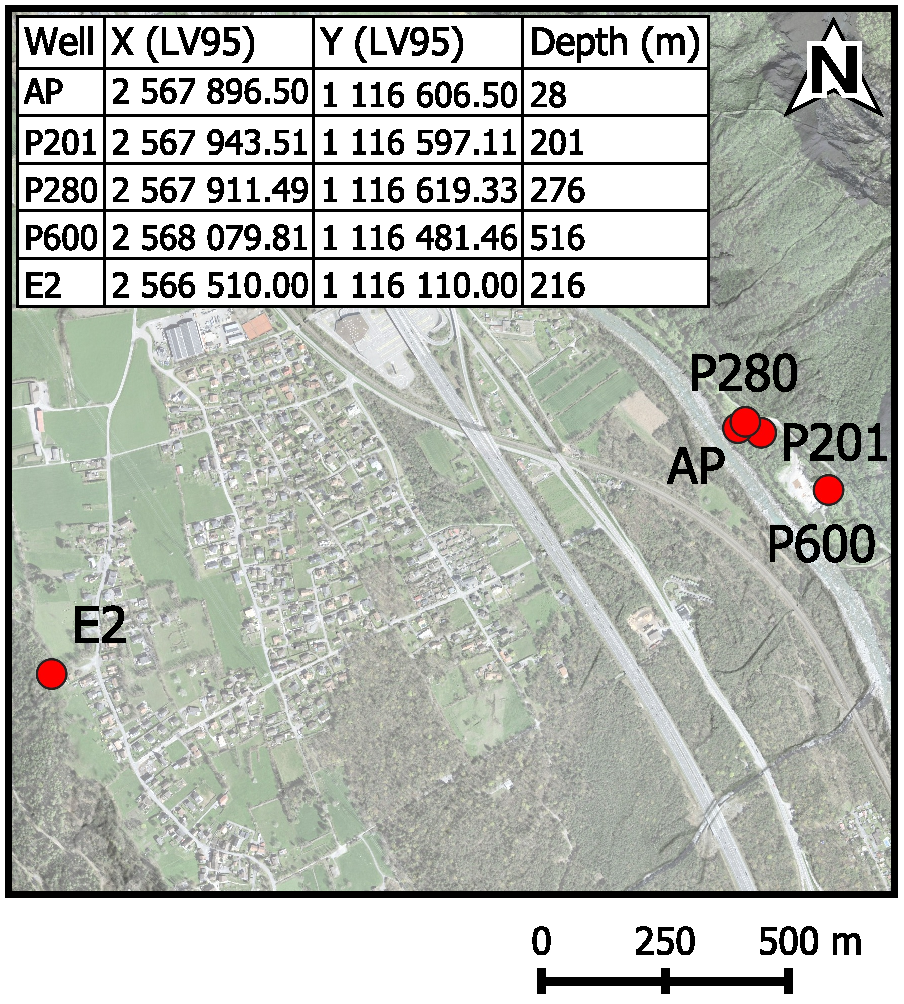
\includegraphics[width=0.8\textwidth]{chapters/06_appendix/SI_C2/Lavey_zoom.pdf}
\caption{Site location of the major wells of Lavey-les-Bains (AP, P201, P280, and P600) and Epinassey (E2) used in this studies.
Map sources: satellite imagery \citep{swisstopo2024swissimage}; digital elevation model \citep{swisstopo2024swissalti3D}; EPSG:3035.}
\label{figSI:map_Lavey}
\end{figure}
\vfill 
\end{center}

\newpage
\null
\vfill
\begin{figure}[H]
\centering
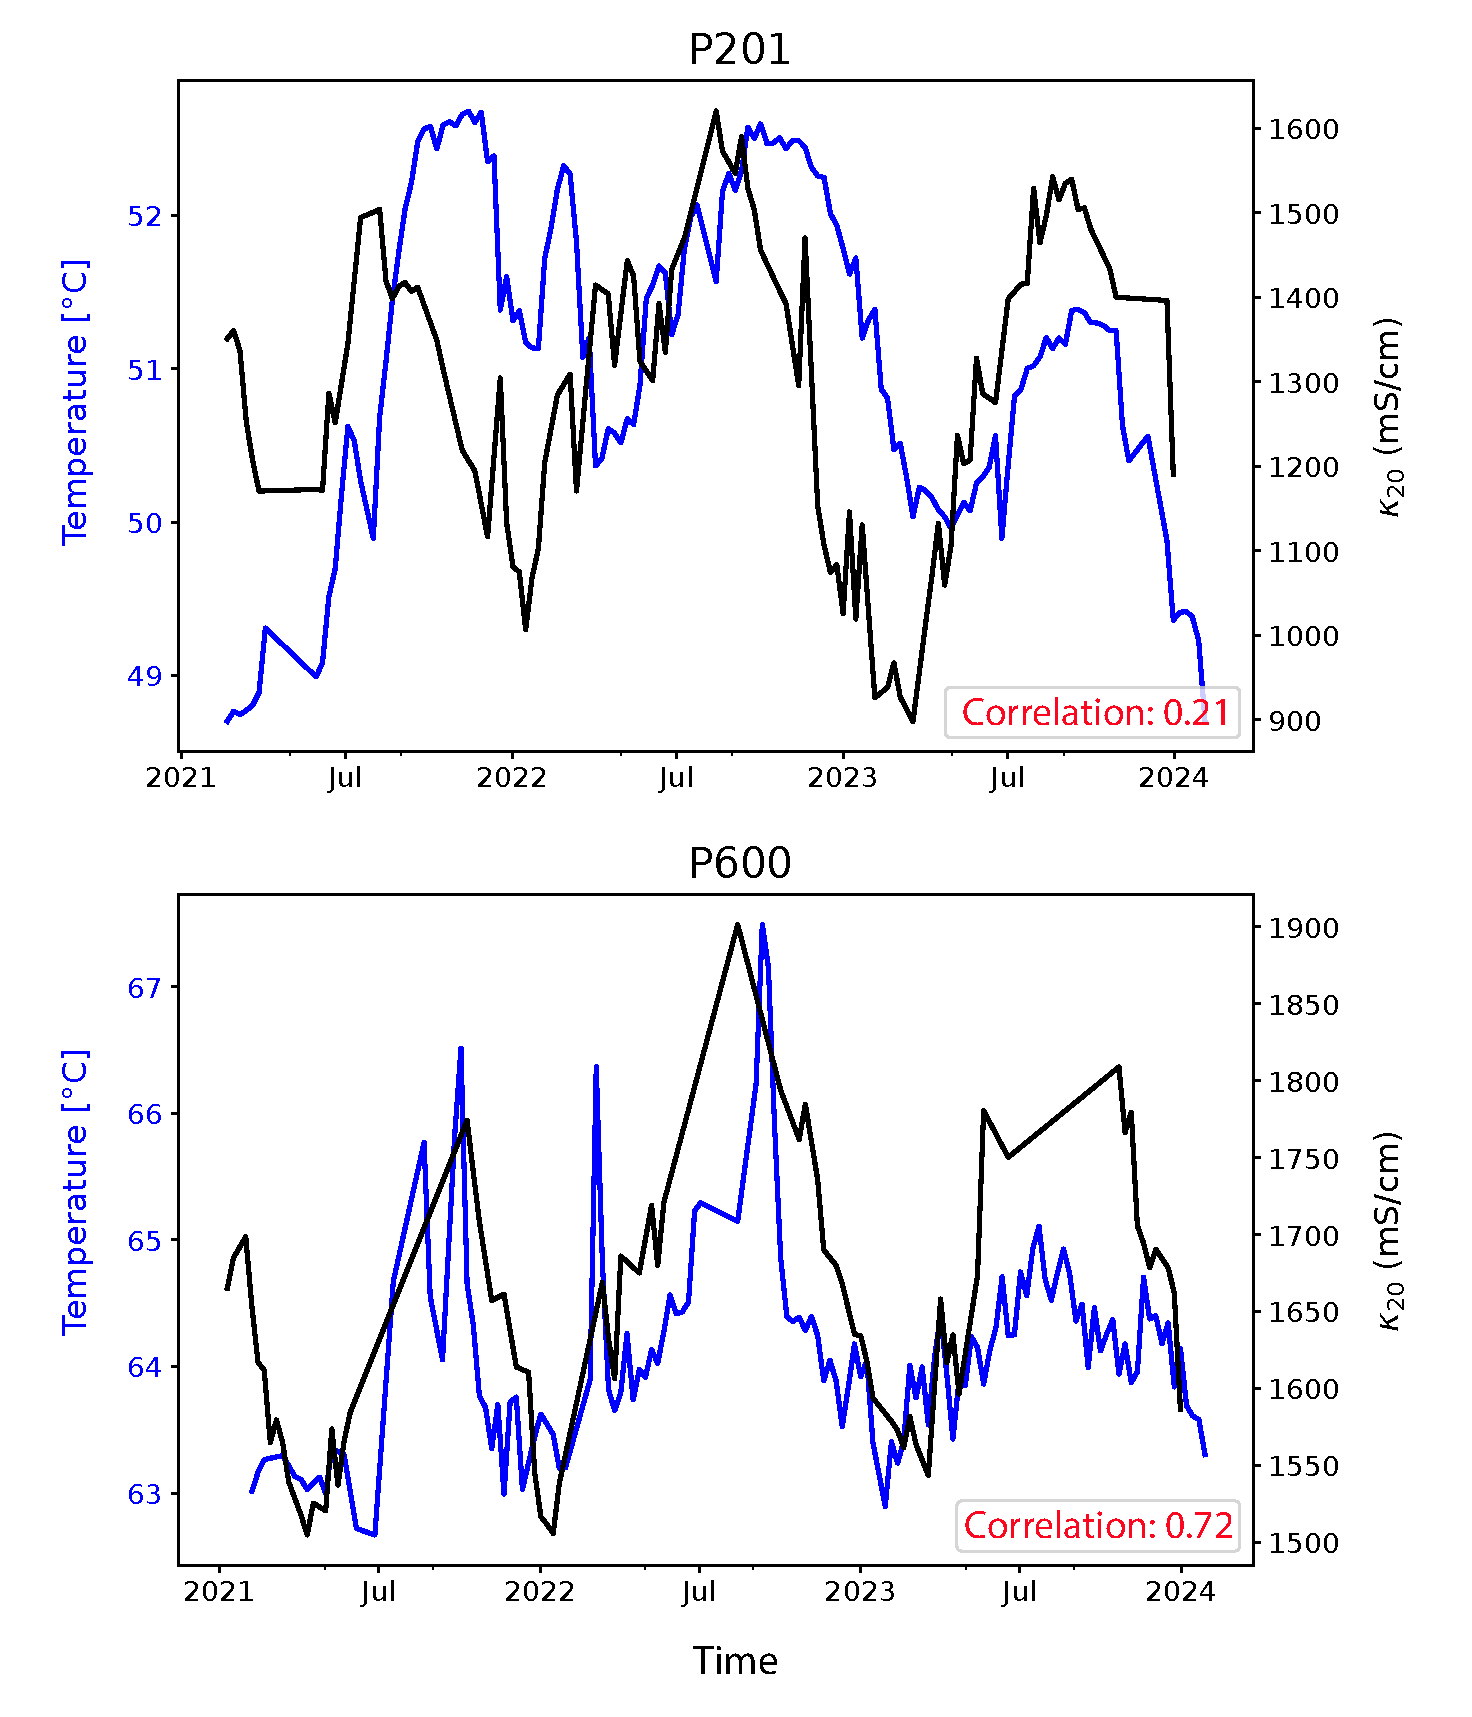
\includegraphics[width=0.8\textwidth]{chapters/06_appendix/SI_C2/EC_vs_temp.pdf}
\caption{Temporal evolution of weekly electrical conductivity and weekly averaged temperature measurements in wells P201 (\textit{top}) and P600 (\textit{bottom}).
The correlation between electrical conductivity and temperature in the case of the P600 is high, highlighting the seasonal mixing between the deep and shallower water component. 
The correlation is less pronounced for the P201, indicating an additional water input in the thermal system.
}
\label{figSI:EC_vs_temp}
\end{figure}
\vfill 


\begin{sidewaysfigure}
\begin{figure}[H]
    \centering
    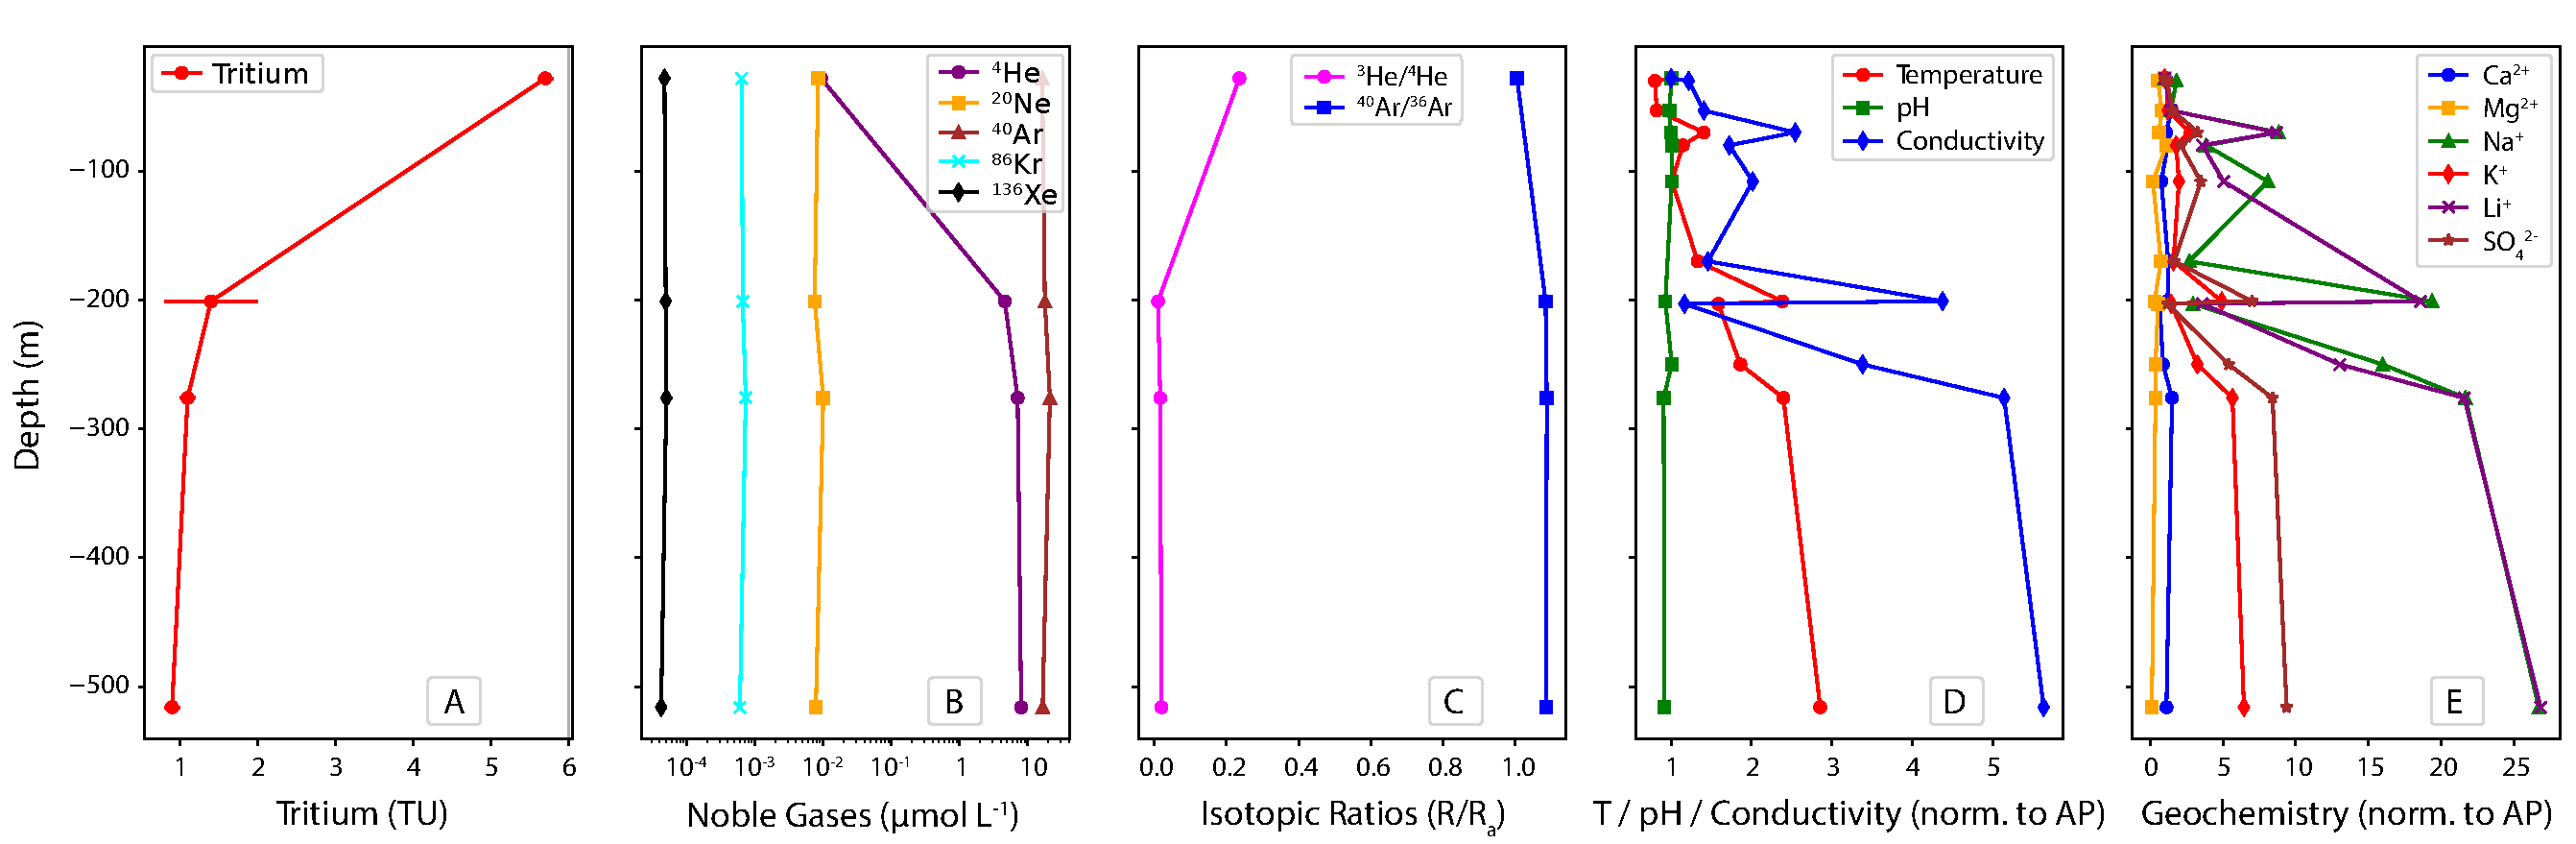
\includegraphics[width=1\textwidth]{chapters/06_appendix/SI_C2/geochemistry_full_plot.pdf}
    \caption{Integrated geochemical and isotopic analysis of thermal waters from Lavey-les-Bains.
    This figure presents a comprehensive dataset from three key boreholes (Table~1), showing: 
    (A) tritium concentrations in tritium units (TU), 
    (B) dissolved noble gas concentrations (\SI{}{\micro\mole\per\litre}), including \ce{^4He}, \ce{^{20}Ne}, \ce{^{40}Ar}, \ce{^{86}Kr}, and \ce{^{136}Xe}, 
    (C) isotope ratios \ce{^3He}/\ce{^4He} and \ce{^{40}Ar}/\ce{^{36}Ar}, normalized by the respective atmospheric ratio \ce{R_a}, 
    (D) profiles of temperature, pH, and electrical conductivity, and 
    (E) major ion concentrations (\ce{Ca^{2+}}, \ce{Mg^{2+}}, \ce{Na+}, \ce{K+}, \ce{Li+}, \ce{SO4^{2-}}).
    Graphs (D) and (E) are normalized to the surface well to highlight depth-related variations in the thermal system.
    These measurements indicate significant thermal water infiltration through fractures in wells P201, P280, and P600, as detailed in Table~1 and supplemented by data from the BDF Geotherm Database \citep{sonney2010database}. 
    The exact values and averages used in plots D and E are provided in Supplementary Datasheet S12 for reference.}
    \label{figSI:geochemistry}
\end{figure}
\end{sidewaysfigure}

\newpage
\null
\vfill
\begin{figure}[H]
\centering
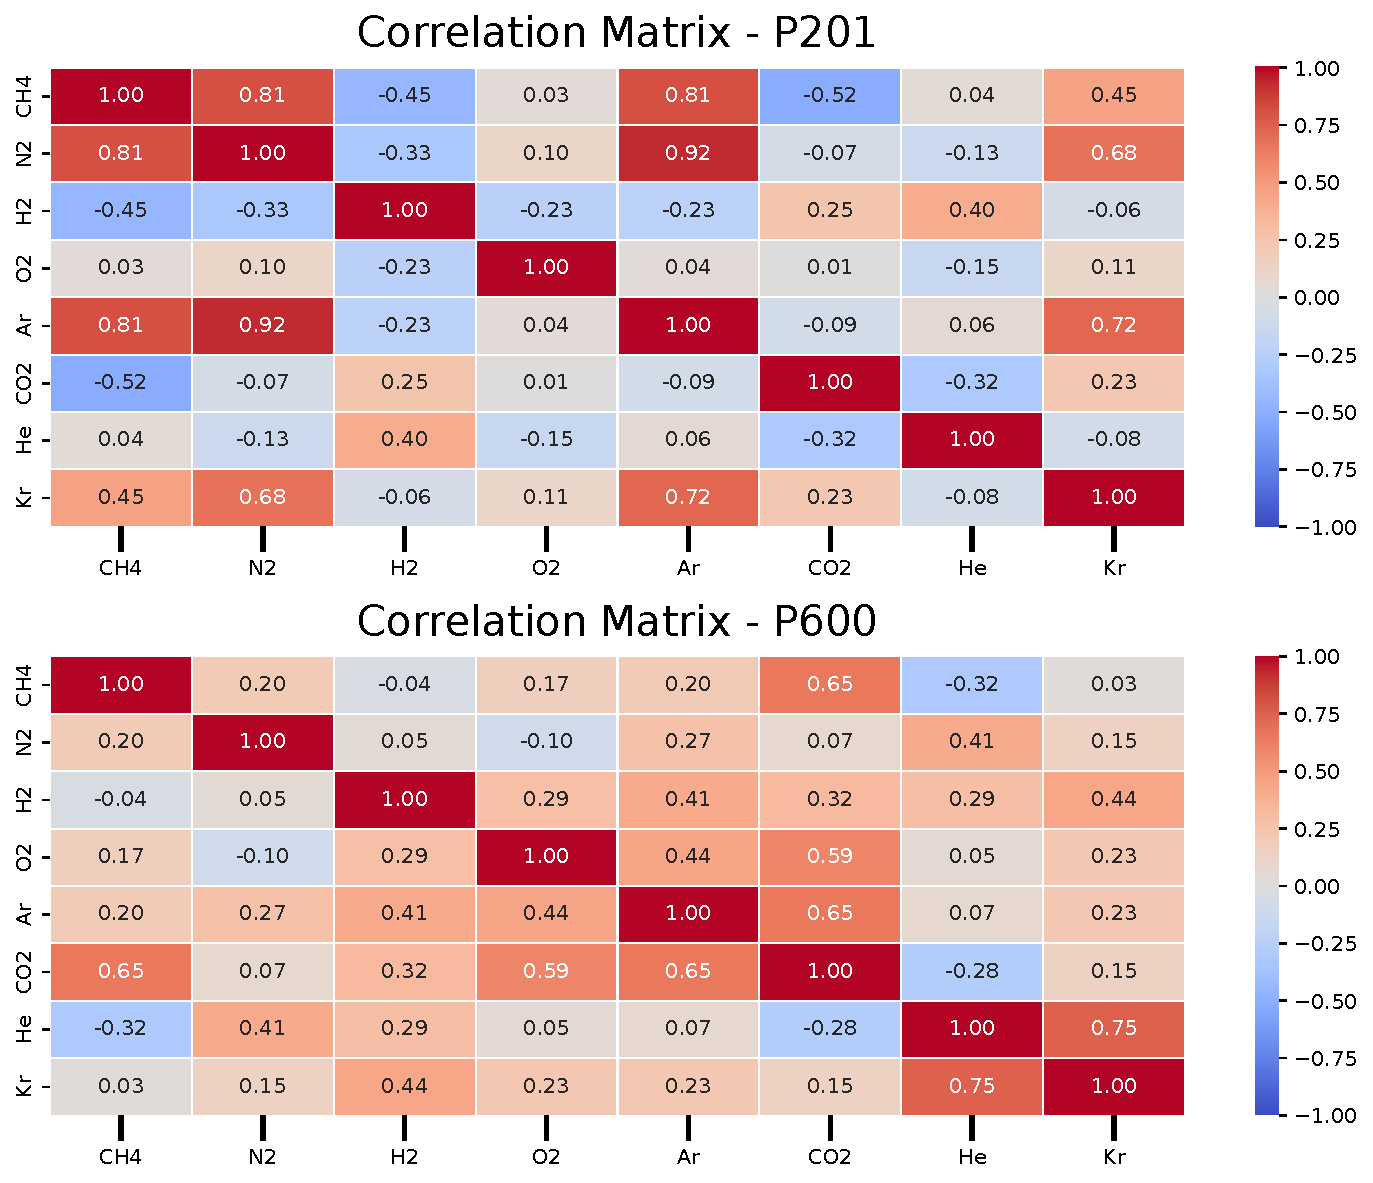
\includegraphics[width=0.8\textwidth]{chapters/06_appendix/SI_C2/correlation_plot.pdf}
\caption{Correlation analysis of the data from the miniRUEDI monitoring in Lavey-les-Bains. 
The correlation matrix for the well P201 (\textit{above}) shows a strong correlation between atmospheric components, such as \ce{N2} and Ar, and \ce{CH4}. 
This suggests that \ce{CH4} is entering the thermal system with an aquifer close to the surface.
In comparison, the correlation matrix for the well P600 (\textit{below}) shows a different relation.
In the deeper section of the thermal system, \ce{CH4} is correlating with \ce{CO2}, which implies a common "deep" source of these geogenic gases. 
}
\label{figSI:correlation}
\end{figure}
\vfill 

\newpage
\null
\vfill
\begin{figure}[H]
\centering
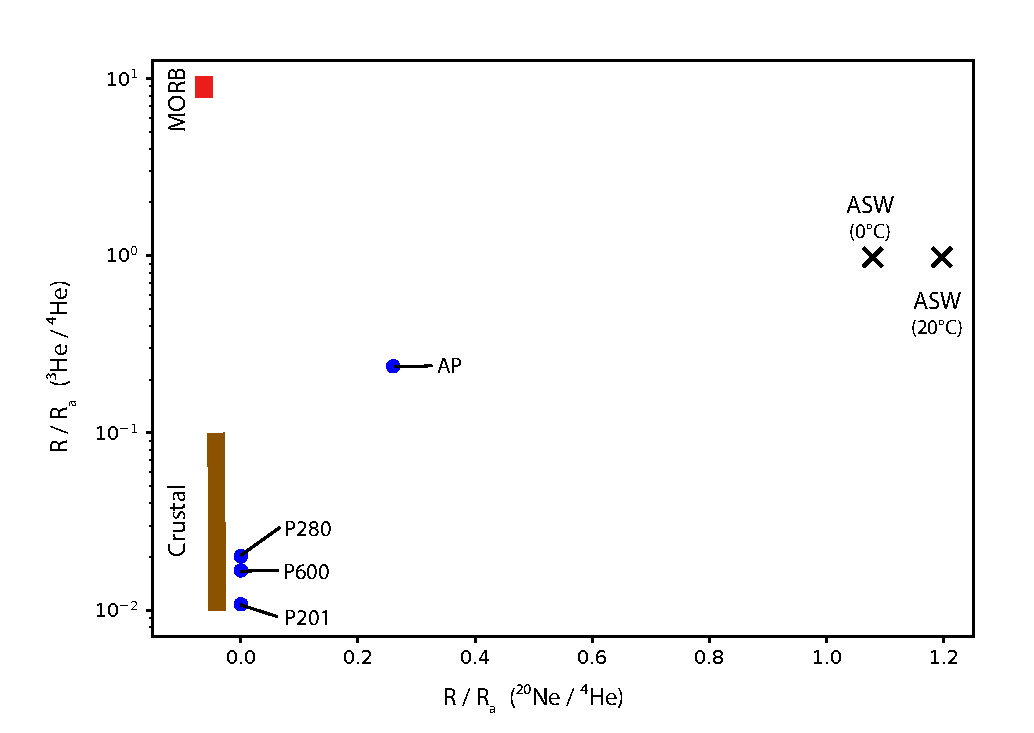
\includegraphics[width=0.8\textwidth]{chapters/06_appendix/SI_C2/Ne20-He3-He4.pdf}
\caption{
\ce{^3He}/\ce{^4He} vs. \ce{^{20}Ne}/\ce{^4He} plot of the samples taken in Lavey-les-Bains.
Ratios are normalized to the respective atmospheric ratios (R$_a$).
The \ce{^3He}/\ce{^4He} ratios typical for mid-ocean ridge basalts (MORB) and radiogenic continental rocks (crustal) are indicated by sidebars, providing a reference for mantle and crustal contributions \citep{lupton1983terrestrial}.
Samples from Lavey-les-Bains are clearly in the crustal range.
Additionally, air saturated water (ASW) at \SI{0}{\celsius} and \SI{20}{\celsius} are represented by two crosses.
}
\label{figSI:NeHe_plot}
\end{figure}
\vfill 

\newpage
\null
\vfill
\begin{figure}[H]
\centering
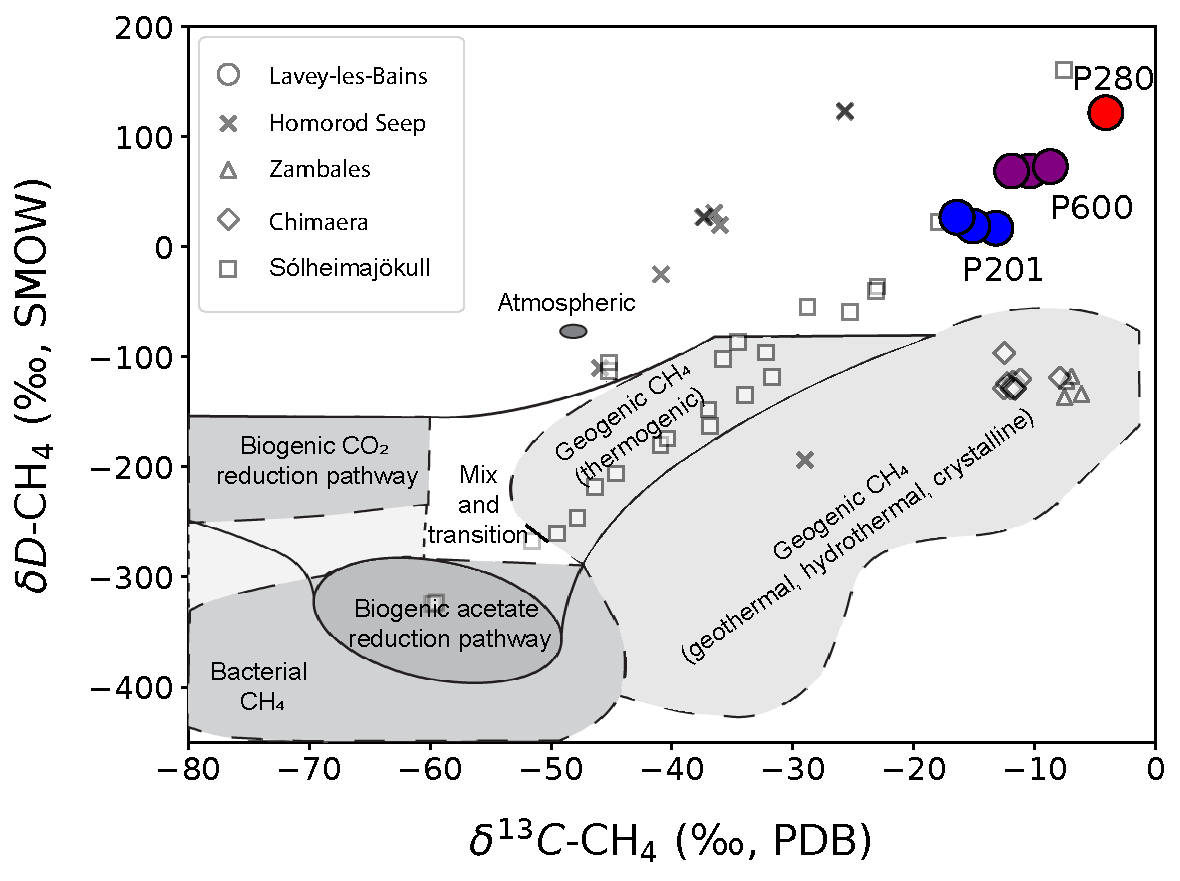
\includegraphics[width=0.8\textwidth]{chapters/06_appendix/SI_C2/CD-plot.pdf}
\caption{
Carbon-hydrogen (\ce{C}-\ce{D}) isotope diagram of \ce{CH4}, modified from \citep{burns2018isotopes}.
The $\delta$-D and $\delta$-\ce{^{13}C} values of \ce{CH4} sampled from wells P201, P280, and P600 are isotopically heavy, suggesting oxidation-derived \ce{CH4} of abiotic origin.
For comparison, similar samples from mud volcanoes in Transylvania (Romania; Homorod Seep 3 \& 4, \cite{etiope2011homorod}), gas seeps in the Philippines (Zambales ophiolite, \cite{abrjano1988zambales}), and Turkey (Chimaera seep and Tekirova ophiolites, \cite{etiope2011chimaera}), as well as geothermal and glacial environments in Iceland (Sólheimajökull glacier, \cite{burns2018isotopes}), are included.
}
\label{figSI:CD_plot}
\end{figure}
\vfill 

\newpage
\null
\vfill
\begin{figure}[H]
\centering
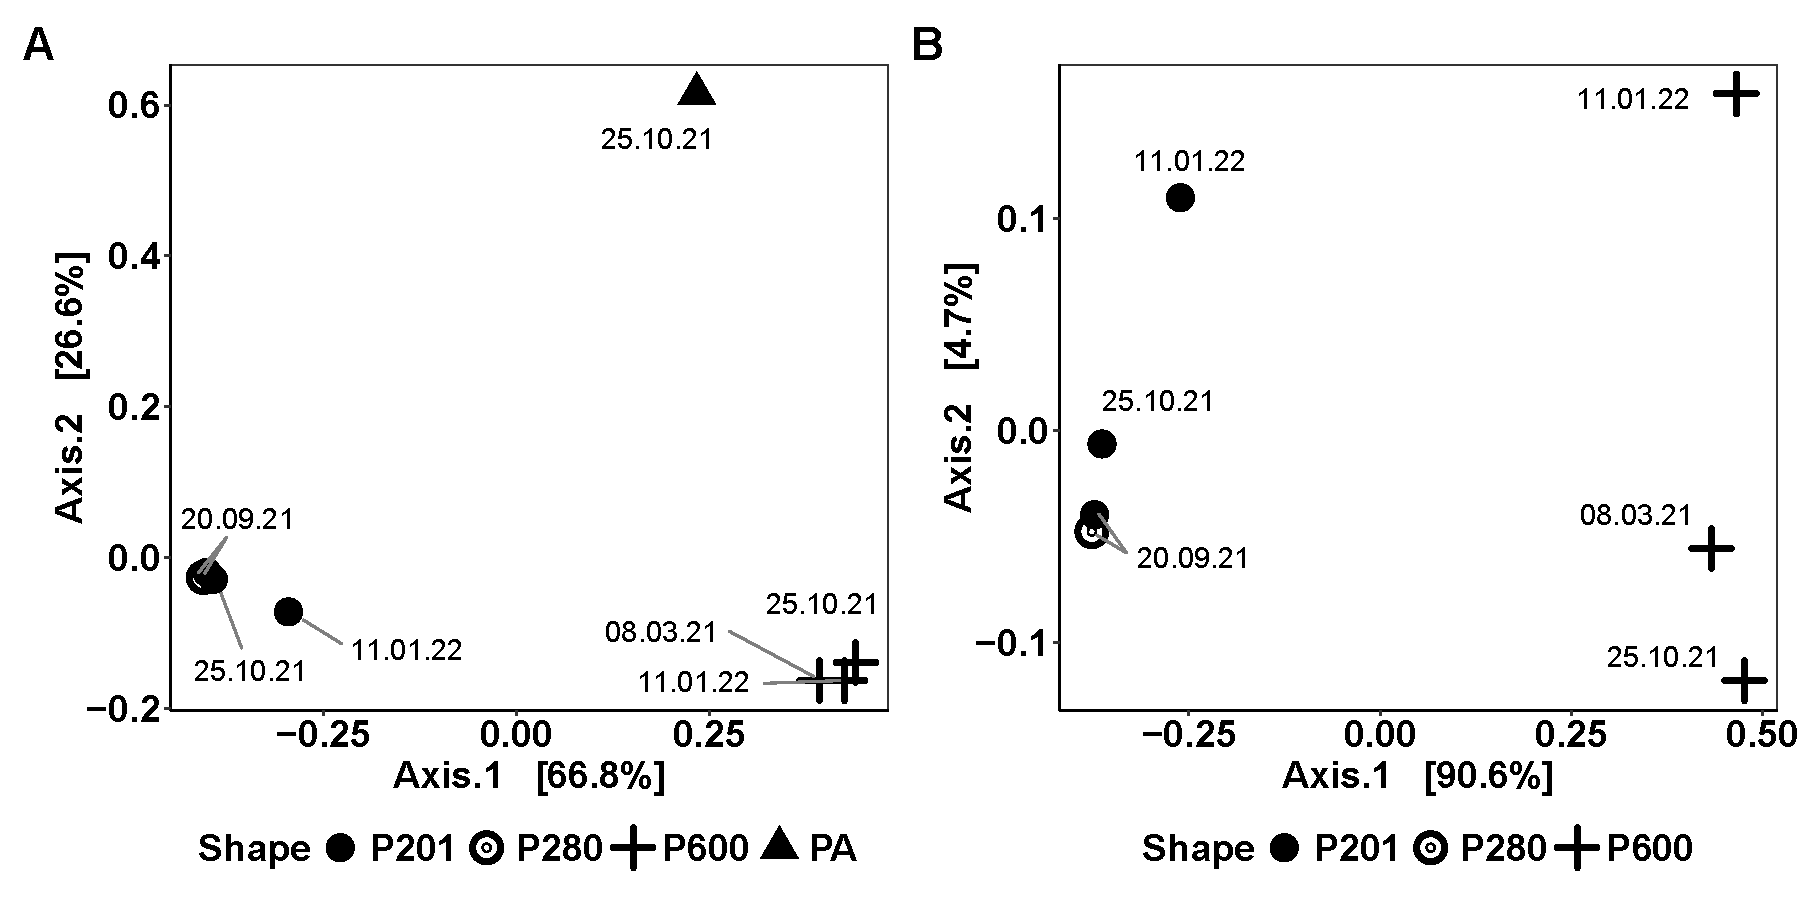
\includegraphics[width=\textwidth]{chapters/06_appendix/SI_C2/PCoA_arc_wuni_all_OTUs.pdf}
\caption{Principal Coordinates Analysis (PCoA) of archaeal communities at the ZOTU level for Lavey-les-Bains using a weighted UniFrac distance matrix. The PCoA shows the separation of the different microbial communities based on their depth.
\textit{A}: Includes all four wells, with P201 and P600 sampled three times over the study period. Both axes show a relatively high degree of separation between surface (AP), intermediate (P201 and P280), and deep (P600) archaeal communities.
\textit{B}: Focuses on the three deep wells, highlighting temporal stability in community structure for P201 and P600. Axis 1 shows the greatest degree of separation, with about \SI{70}{\percent} of the variance between communities from intermediate depths (P201 and P280) and the deep layer (P600).}
\label{figSI:PCoA_arc}
\end{figure}
\vfill 

\newpage
\null
\vfill
\begin{figure}[H]
\centering
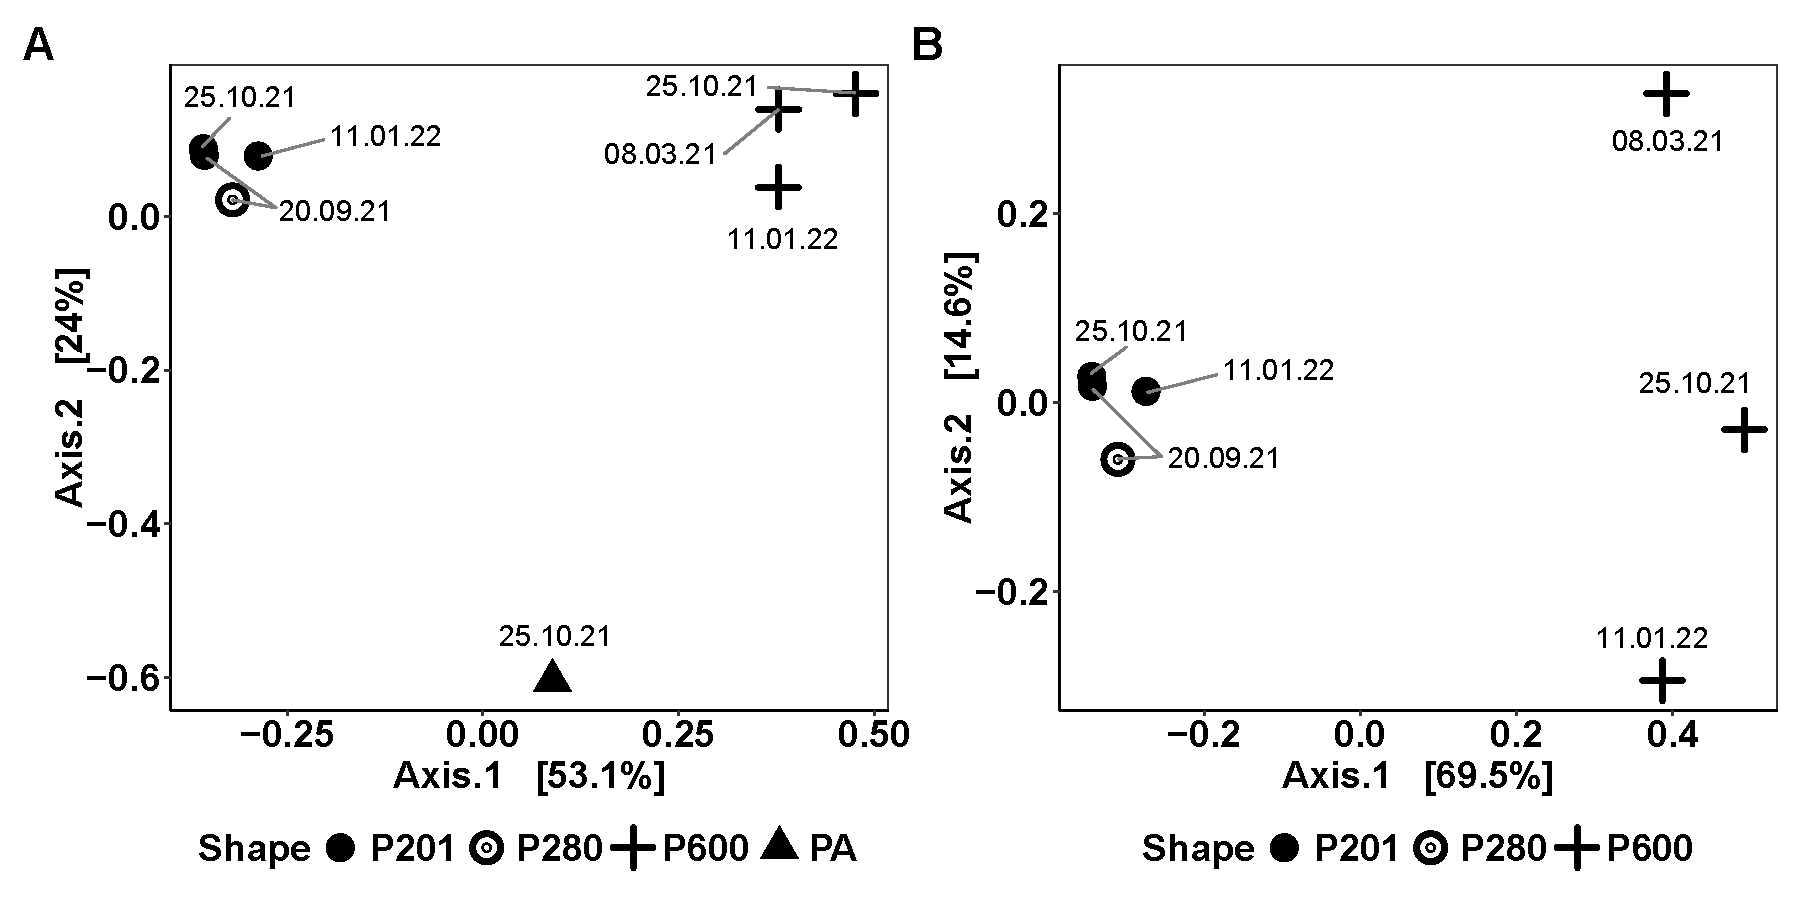
\includegraphics[width=\textwidth]{chapters/06_appendix/SI_C2/PCoA_bac_wuni_all_OTUs.pdf}
\caption{Principal Coordinates Analysis (PCoA) of bacterial communities at the ZOTU level for Lavey-les-Bains using a weighted UniFrac distance matrix. The PCoA shows the separation of the different microbial communities based on their depth.
\textit{A}: Includes all four wells, with P201 and P600 sampled three times over the study period. Both axes show a relatively high degree of separation between surface (AP), intermediate (P201 and P280), and deep (P600) bacterial communities.
\textit{B}: Focuses on the three deep wells, highlighting temporal stability in community structure for P201 and P600. Axis 1 shows the greatest degree of separation, with about \SI{70}{\percent} of the variance between communities from intermediate depths (P201 and P280) and the deep layer (P600).}
\label{figSI:PCoA_bac}
\end{figure}
\vfill 

\newpage
\null
\vfill
\begin{figure}[H]
\centering
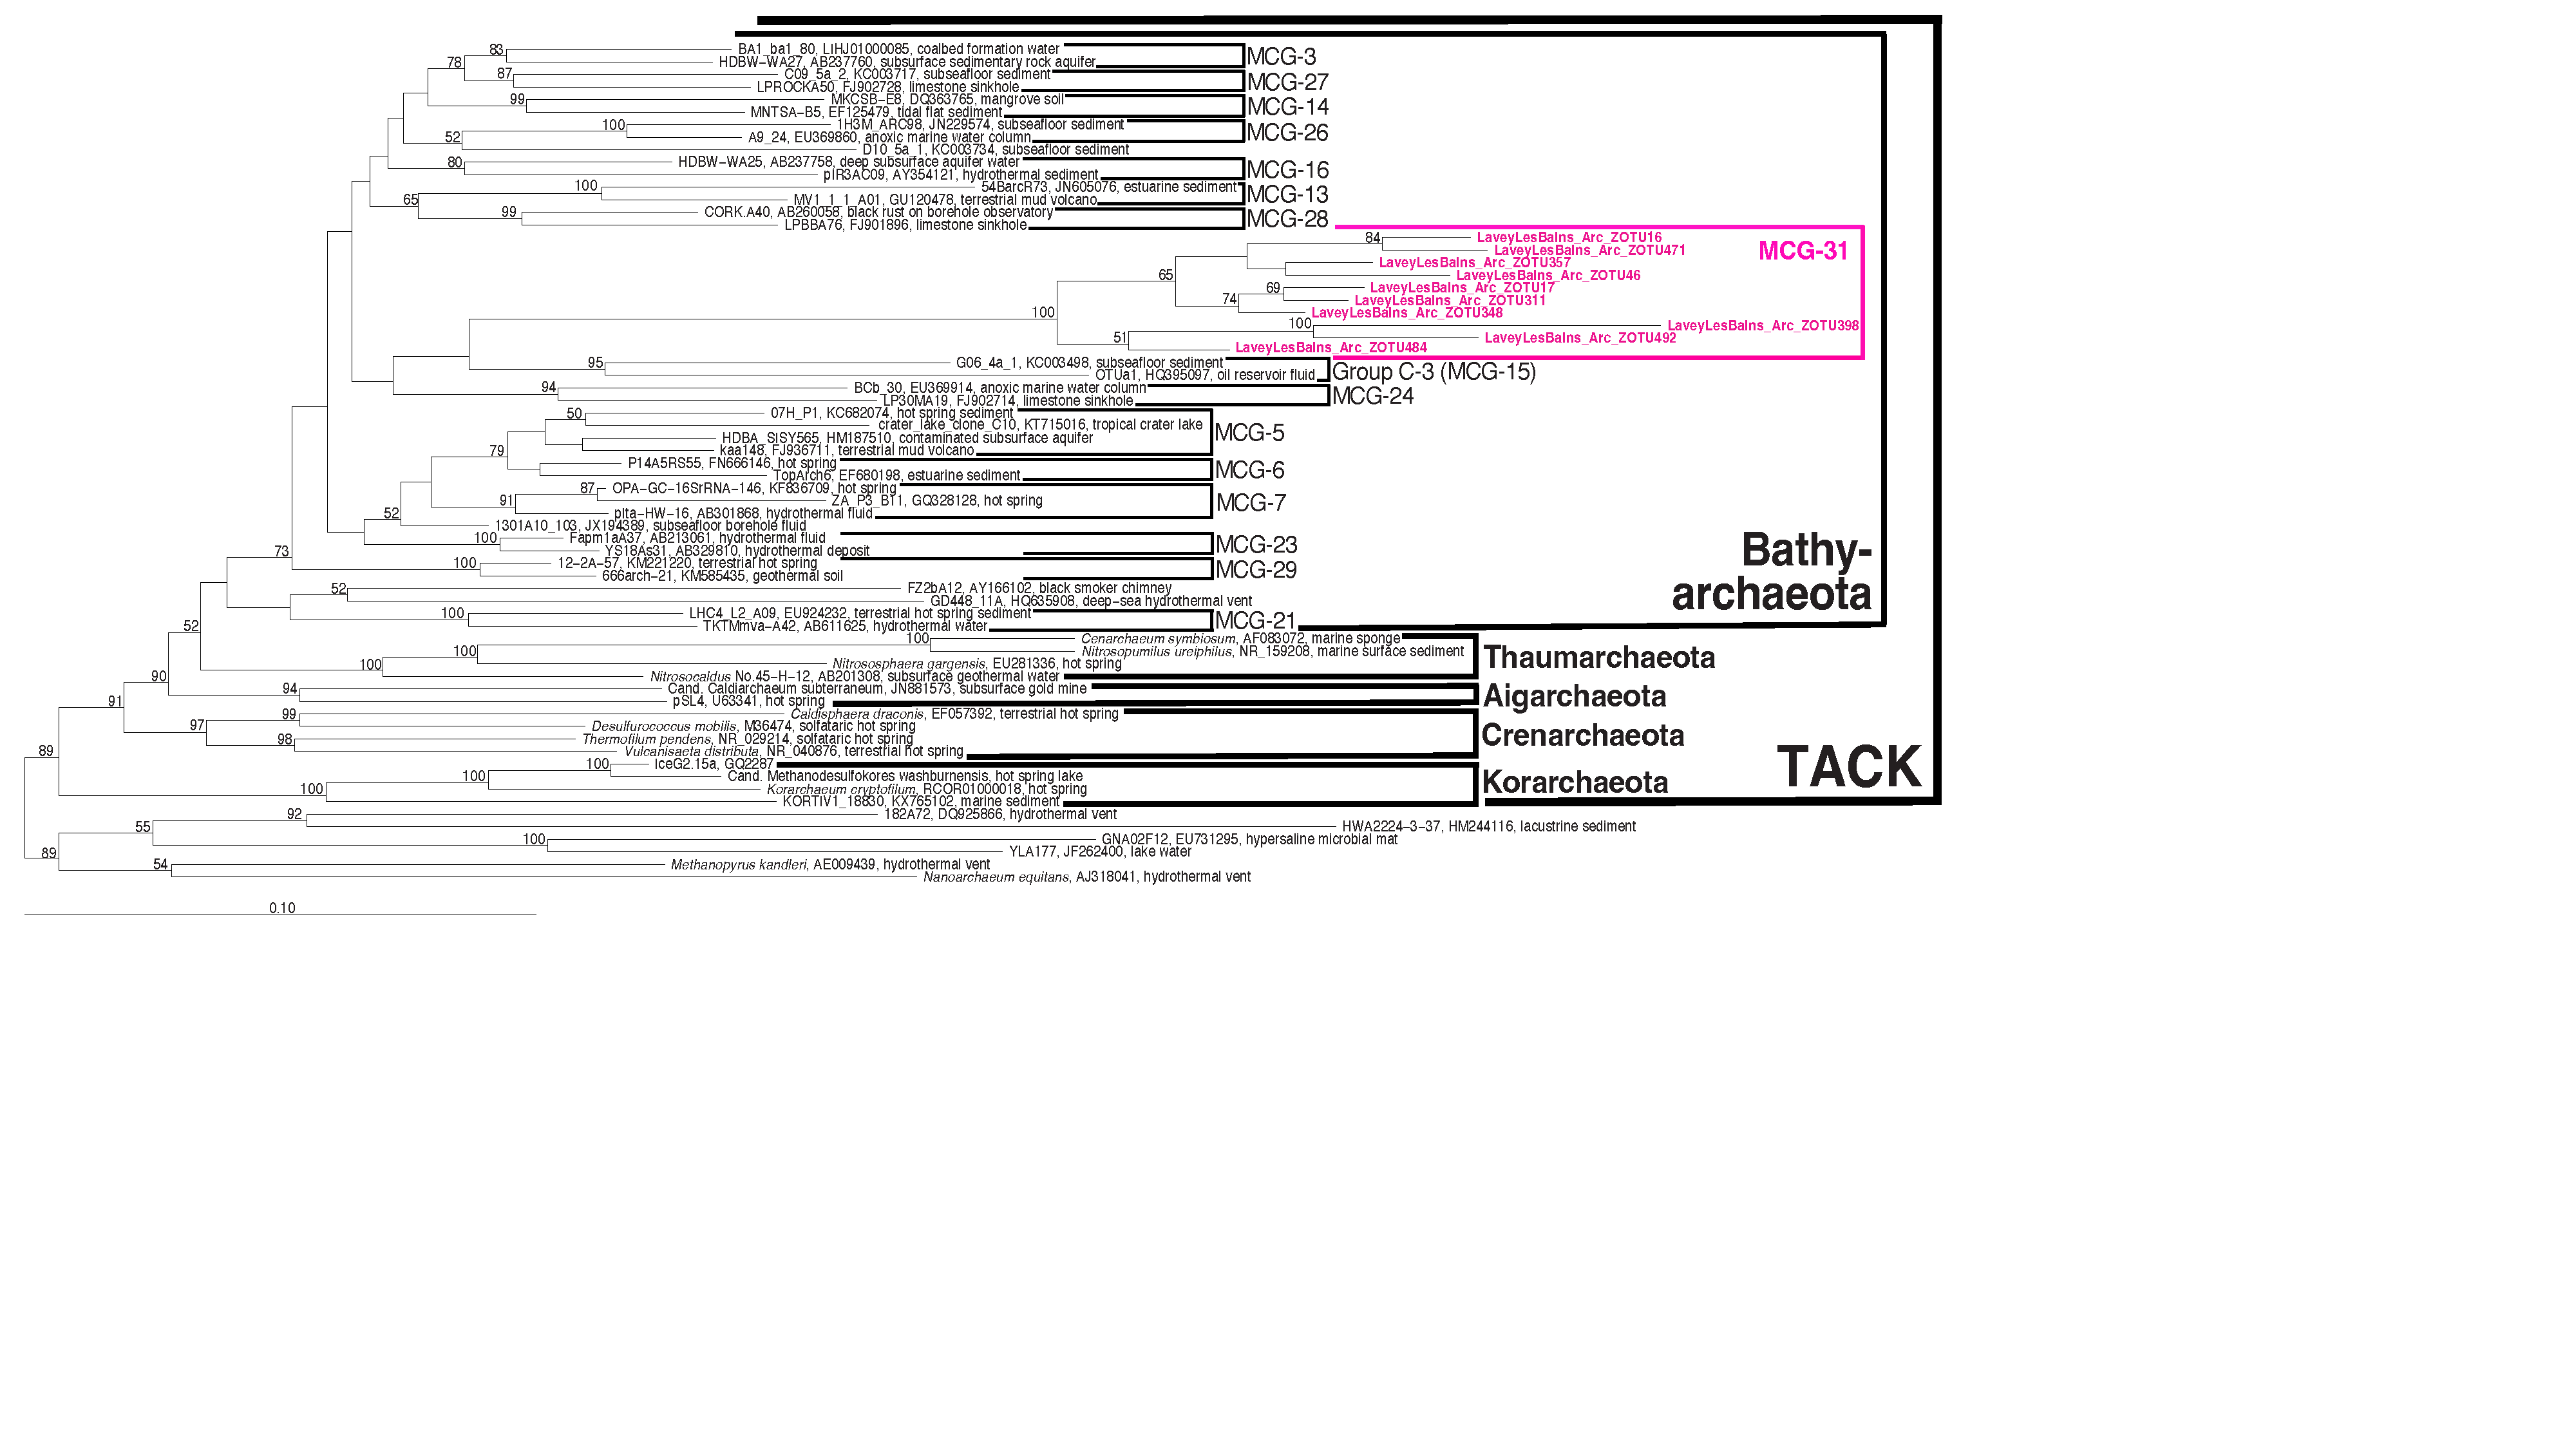
\includegraphics[width=\textwidth]{chapters/06_appendix/SI_C2/LLB_NewBathyarchaeotaGroup.pdf}
\caption{
Phylogenetic tree showing novel, deeply-branching Bathyarchaeaota cluster (MCG-31), as well as related phyla, which together with Bathyarchaeota make up the TACK superphylum.
The phylogenetic tree was constructed using ARB Neighbor Joining (Jukes-Cantor Correction) within the ARB software and is based on manually optimized 16S rRNA gene sequence alignments.
}
\label{figSI:MCG31}
\end{figure}
\vfill 

\newpage
\null
\vfill
\begin{figure}[H]
\centering
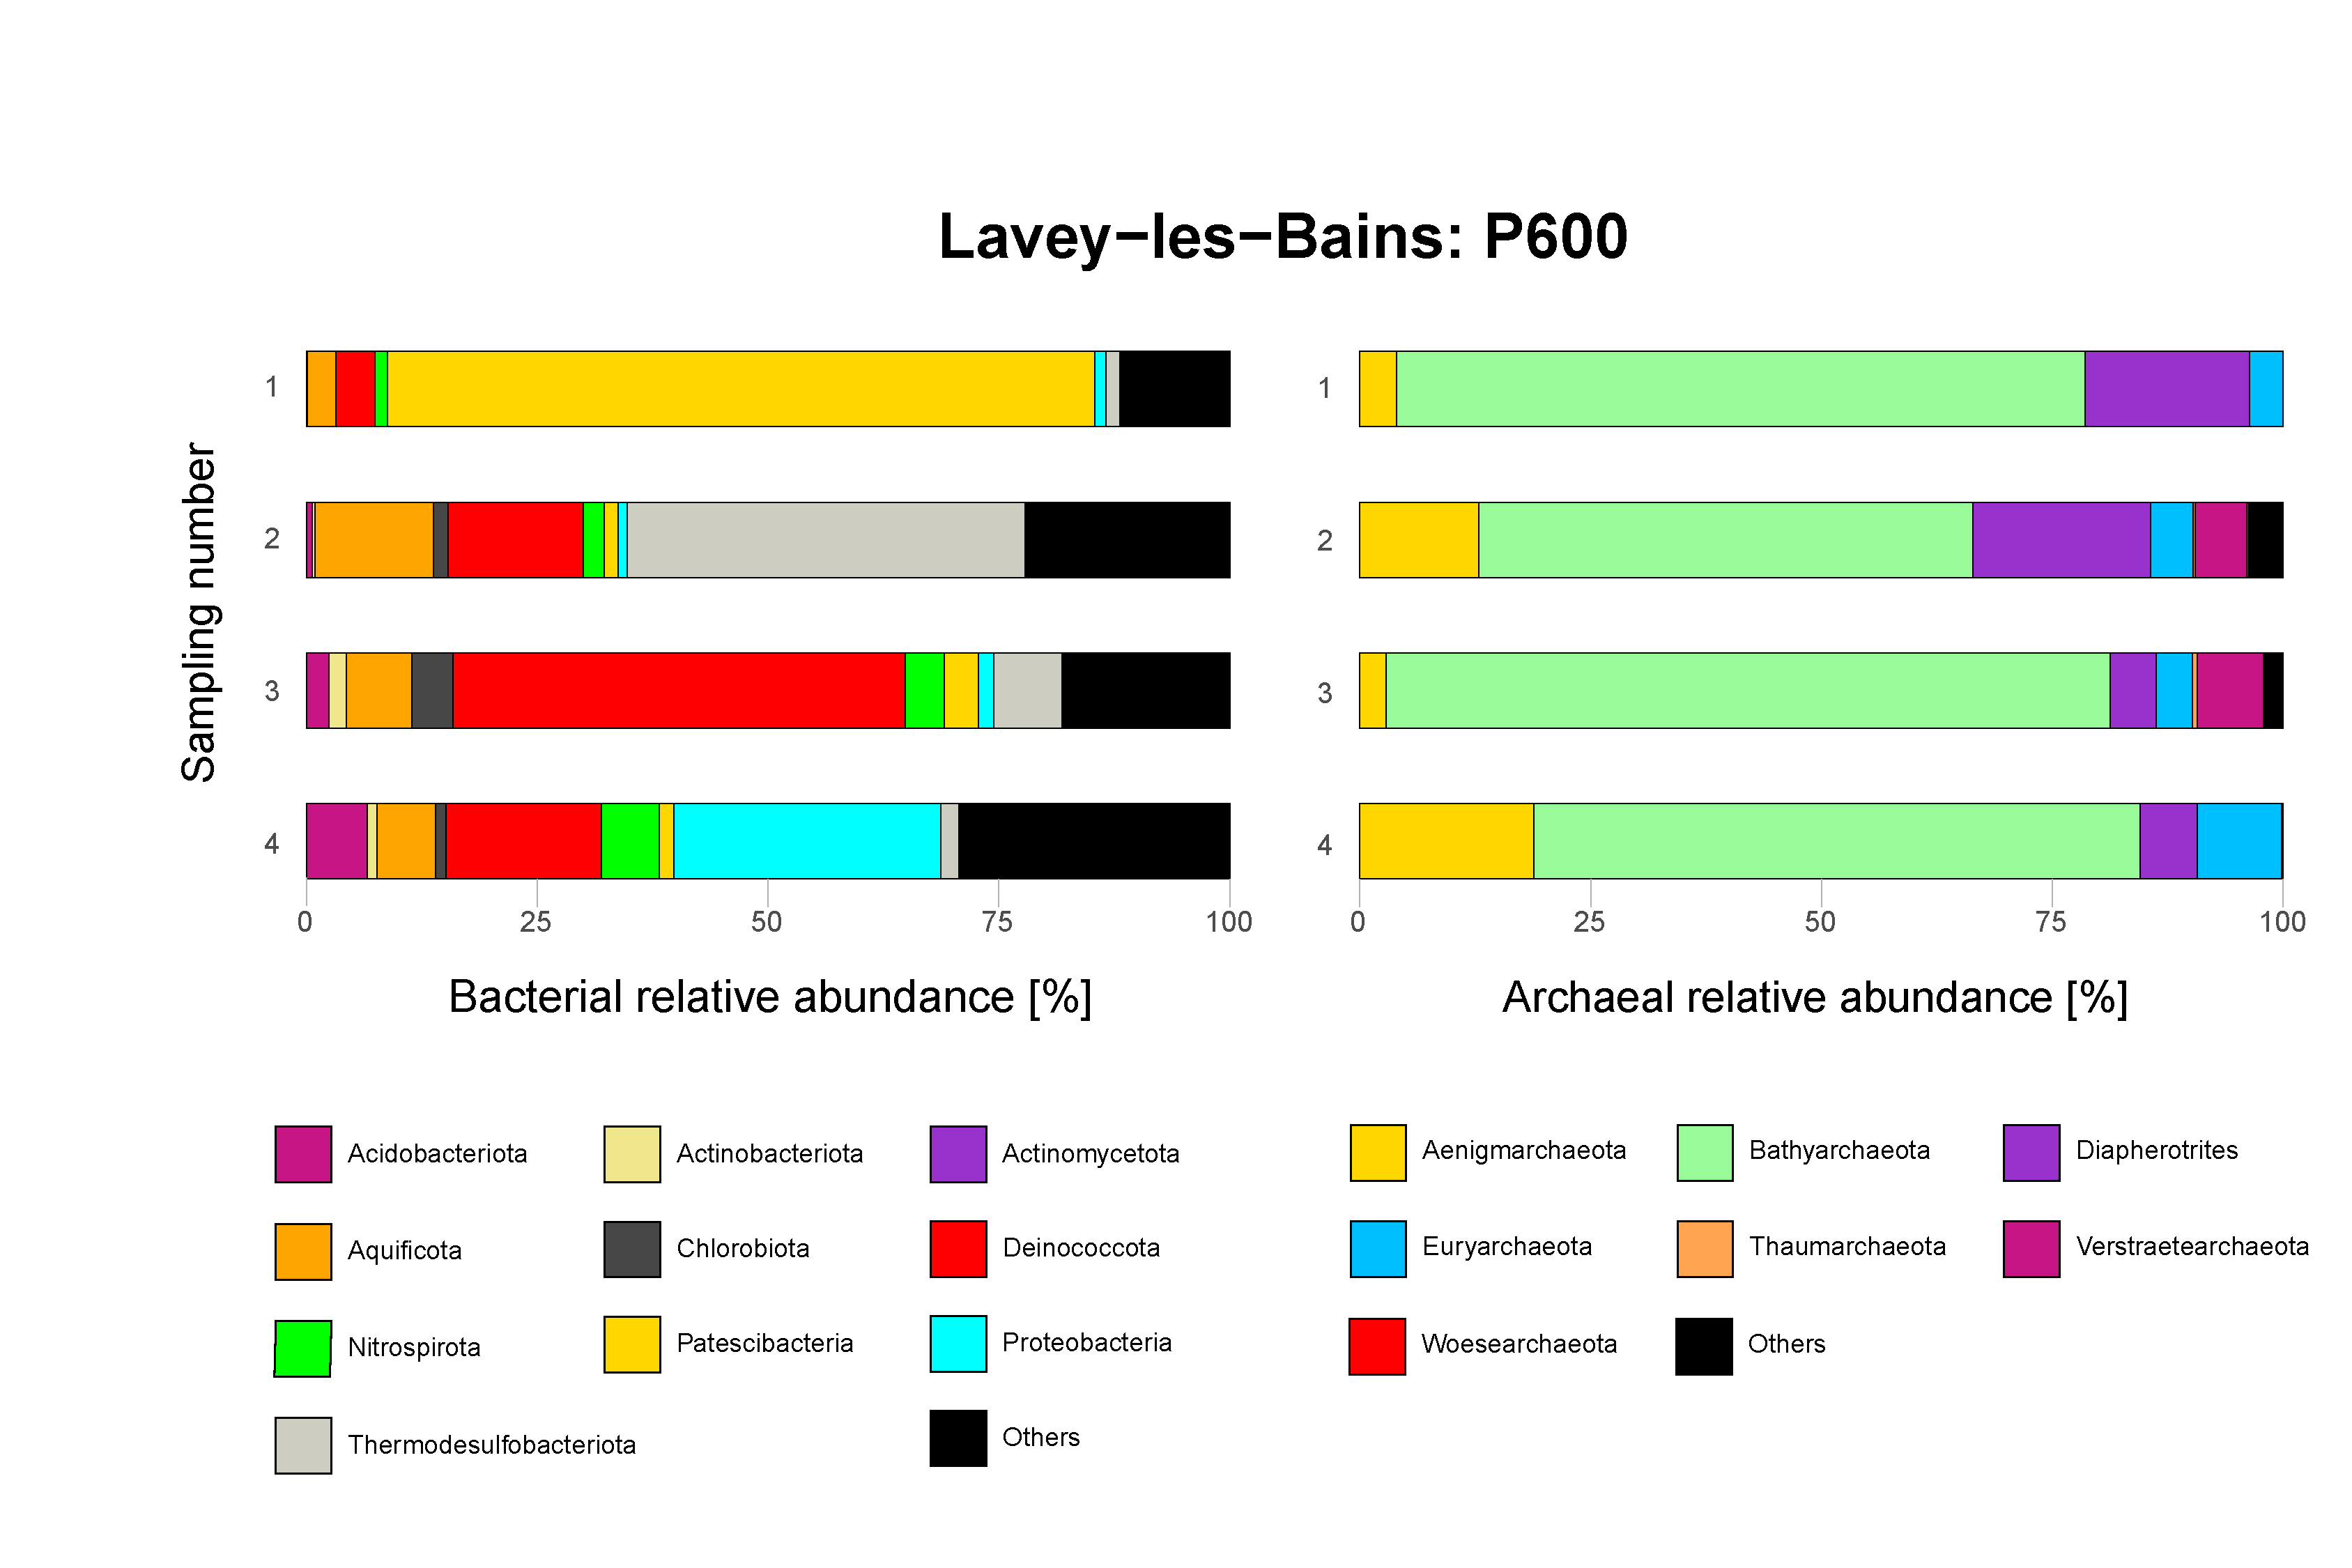
\includegraphics[width=\textwidth]{chapters/06_appendix/SI_C2/phylum_test_Lavey.pdf}
\caption{
This figure illustrates the microbial relative abundances in well P600 of Lavey-les-Bains.
Sampling numbers 2 to 4 are presented in the main body of the article.
Sampling number 1 was part of the initial testing phase, where a sequential filtration process was used (\SI{0.2}{\micro\metre} cellulose acetate filtration, followed by \SI{0.1}{\micro\metre} polyethersulfone filtration).
Due to the non-dissolution of the cellulose acetate, the microbial community fraction larger than \SI{0.2}{\micro\metre} was lost.
However, the recovered and successfully identified \SI{0.1}{\micro\metre} microbial community revealed the presence of members from DPANN (Diapherotrites), the proposed deep-branching Bathyarchaeota cluster MCG-31 (Unclassified Archaea I), and the candidate phyla radiation (Patescibacteria), highlighting the importance of using \SI{0.1}{\micro\metre} filtration.
}
\label{figSI:filter_comp}
\end{figure}
\vfill 

\newpage

\section{Tables}
\begin{center}
\vfill
\begin{table}[H]
\centering
\begin{adjustbox}{width=0.5\textwidth}
\caption{Stable water isotopes measurement from Salvan's spring and Lavey-les-Bains' wells from 21-25.08.2021. Isotopic results are noted in the standard $\delta$-notation relative to Vienna Standard Mean Ocean Water (VSMOW). Precision of measurements are given by the standard deviation (SD) of multiple injections.}
\label{tabSI:stables_Salvan}
\renewcommand{\arraystretch}{2.5}
\sisetup{
    scientific-notation = true,
    round-mode = figures,
    round-precision = 3
}
\footnotesize
\begin{tabular}{@{}lccccc@{}}
\toprule
Sample & Location & {$\delta$\ce{^{18}O}} & SD & {$\delta$\ce{^{2}H}} & SD  \\
\midrule
Tende                   & les Marécottes  & -12.3 & 0.01 & -89.9 & 0.07 \\
Peutex                  & les Marécottes  & -13.0 & 0.01 & -93.5 & 0.09 \\
Creusaz                 & les Marécottes  & -12.8 & 0.01 & -90.5 & 0.02 \\
Mialley                 & Van d'en Haut   & -12.2 & 0.01 & -86.6 & 0.03 \\
Plan les Diés           & Van d'en Haut   & -12.6 & 0.02 & -90.2 & 0.04 \\
Galerie CFF pompage     & les Granges     & -12.5 & 0.56 & -92.2 & 1.56 \\
Revenasse               & les Marécottes  & -12.9 & 0.02 & -93.0 & 0.03 \\
Abérieu                 & Trétien         & -12.8 & 0.01 & -91.4 & 0.03 \\
P201                    & Lavey-les-Bains & -12.9 & 0.02 & -93.8 & 0.03 \\
AP                      & Lavey-les-Bains & -12.0 & 0.01 & -86.5 & 0.08 \\
P600                    & Lavey-les-Bains & -13.2 & 0.02 & -96.3 & 0.09 \\
\bottomrule
\end{tabular}
\end{adjustbox}
\end{table}
\vfill
\end{center}

\begin{center}
\vfill
\begin{table}[H]
\centering
\begin{adjustbox}{width=0.8\textwidth}
\caption{Dissolved noble gases concentration of water samples from the different boreholes. The measurements are typically in the measuring range given by the miniRUEDI measurements.
Measurement uncertainties were \SI{0.7}{\percent} for \ce{^4He}, \SI{1.2}{\percent} for \ce{^{20}Ne}, \SI{0.8}{\percent} for \ce{^{40}Ar}, \SI{1.0}{\percent} for \ce{^{86}Kr}, and \SI{1.3}{\percent} for \ce{^{136}Xe}.
Uncertainties for \ce{^3H} are provided in the table.}
\label{tabSI:noble_gases}
\renewcommand{\arraystretch}{2.5}
\sisetup{
    scientific-notation = true,
    round-mode = figures,
    round-precision = 2
}
\footnotesize
\begin{tabular}{@{}lcccccc@{}}
\toprule
Borehole & \ce{^4He} [\SI{}{\umol\per\liter}] & \ce{^{20}Ne} [\SI{}{\umol\per\liter}] & \ce{^{40}Ar} [\SI{}{\umol\per\liter}] & \ce{^{86}Kr} [\SI{}{\umol\per\liter}] & \ce{^{136}Xe} [\SI{}{\umol\per\liter}] & \ce{^3H} (TU) \\
\midrule
AP    & \SI{9.3E-3}{}  & \SI{8.4E-3}{}  & 16.3 & \SI{6.4E-4}{}  & \SI{4.7E-5}{}  & \SI{5.7(1)}{} \\
P201  & \SI{4.6}{}     & \SI{7.5E-3}{}  & 17.8 & \SI{6.6E-4}{}  & \SI{4.9E-5}{}  & \SI{1.4(6)}{} \\
P280  & \SI{7.1}{}     & \SI{1.0E-2}{}  & 21.1 & \SI{7.3E-4}{}  & \SI{5.0E-5}{}  & \SI{1.1(1)}{} \\
P600  & \SI{8.0}{}     & \SI{7.8E-3}{}  & 16.5 & \SI{6.0E-4}{}  & \SI{4.2E-5}{}  & $0.9 \pm 0.1$ \\
E2    & \SI{5.8E-2}{}  & \SI{8.1E-3}{}  & 16.5 & \SI{6.7E-4}{}  & \SI{5.0E-5}{}  & - \\
\bottomrule
\end{tabular}
\end{adjustbox}
\end{table}
\vfill
\begin{table}[H]
\centering
\begin{adjustbox}{width=0.8\textwidth}
\caption{Isotope ratios of noble gases measured in the different boreholes of Lavey-les-Bains and the control borehole E2.}
\label{tabSI:isotope_ratios}
\renewcommand{\arraystretch}{2.5}
% \sisetup{
%     scientific-notation = true,
%     round-mode = figures,
%     round-precision = 2
% }
\footnotesize
\begin{tabular}{@{}p{2.5cm} m{4cm} m{4cm} m{4cm}@{}}
\toprule
Borehole & {\ce{^3He}/\ce{^4He}} & {\ce{^{20}Ne}/\ce{^{22}Ne}} & {\ce{^{40}Ar}/\ce{^{36}Ar}} \\
\midrule
AP       & \SI{3.3(1)E-07}{} & \SI{9.8(1)}{}   & \SI{296.9(3)}{}  \\
P201     & \SI{1.5(6)E-08}{} & \SI{9.9(1)}{}   & \SI{320.2(3)}{}  \\
P280     & * \SI{2.3(20)E-08}{} & \SI{9.8(1)}{}   & \SI{321.2(3)}{}  \\
P600     & \SI{2.8(2)E-08}{} & \SI{9.7(1)}{}   & \SI{320.6(3)}{}  \\
E2       & \SI{7.5(2)E-08}{} & \SI{9.6(1)}{}   & \SI{293.3(5)}{}  \\
\bottomrule
\multicolumn{4}{p{14.5cm}}{\footnotesize * Measurement from the second extraction. \ce{^3He}/\ce{^4He} subject to larger error due to fractionation effects within the first extraction.}
\end{tabular}
\end{adjustbox}
\end{table}
\vfill
\end{center}

\begin{sidewaystable}[H]  % Use sidewaystable to rotate the table
\centering
\begin{adjustbox}{max width=0.8\textwidth, max totalheight=0.85\textheight, keepaspectratio}
\renewcommand{\arraystretch}{1.5} % Adjust row height to fit more content
\footnotesize % Reduce text size slightly for better fit
\caption{Archaeal taxonomic composition (Part 1) of the most abundant taxa, presented as relative percentages for AP, P201, P280, and P600 at the ZOTU level (each entry represents a single ZOTU).
For P201 and P600, the percentages represent the average of three samples.
The no-template controls (NTC-1 and NTC-2) are also included: NTC-1 consists of reads from the site negative control and the laboratory extraction blank, while NTC-2 includes reads from the library preparation negative controls.
The NTCs indicate the relative abundance of the reads compared to the samples and help to assess potential contamination by the respective taxa.
The results show that the most abundant taxa are predominantly from the samples and not from contamination.
\textit{(Continued in Part 2 on the next page.)}}
\label{tabSI:tax_arc_1}
\begin{tabular}{llllllllll||lll}
\toprule
\textbf{ZOTU} & \textbf{Phylum} & \textbf{Class} & \textbf{Order} & \textbf{Family} & \textbf{Genus} & \textbf{AP} & \textbf{P201} & \textbf{P280} & \textbf{P600} & \textbf{Samples} & \textbf{NTC1} & \textbf{NTC2} \\
\midrule
ZOTU70 & Thaumarchaeota & Nitrososphaeria & Nitrosopumilales & - & - & \SI{43.2}{\percent} & \SI{0.1}{\percent} & \SI{0.1}{\percent} & \SI{0.0}{\percent} & \SI{100.0}{\percent} & \SI{0.0}{\percent} & \SI{0.0}{\percent} \\
ZOTU124 & Thaumarchaeota & Nitrososphaeria & Nitrosopumilales & - & - & \SI{11.4}{\percent} & \SI{0.0}{\percent} & \SI{0.1}{\percent} & \SI{0.0}{\percent} & \SI{100.0}{\percent} & \SI{0.0}{\percent} & \SI{0.0}{\percent} \\
ZOTU63 & Thaumarchaeota & Nitrososphaeria & Nitrosopumilales & Nitrosopumilaceae & - & \SI{9.5}{\percent} & \SI{0.0}{\percent} & \SI{0.0}{\percent} & \SI{0.0}{\percent} & \SI{100.0}{\percent} & \SI{0.0}{\percent} & \SI{0.0}{\percent} \\
ZOTU448 & Thaumarchaeota & Nitrososphaeria & SAGMCG & - & - & \SI{8.3}{\percent} & \SI{0.0}{\percent} & \SI{0.0}{\percent} & \SI{0.0}{\percent} & \SI{100.0}{\percent} & \SI{0.0}{\percent} & \SI{0.0}{\percent} \\
ZOTU450 & Woesearchaeota & - & - & - & - & \SI{2.7}{\percent} & \SI{0.0}{\percent} & \SI{0.0}{\percent} & \SI{0.0}{\percent} & \SI{100.0}{\percent} & \SI{0.0}{\percent} & \SI{0.0}{\percent} \\
ZOTU131 & Thaumarchaeota & MBD-A/AK59/FSCG & - & - & - & \SI{2.6}{\percent} & \SI{0.0}{\percent} & \SI{0.0}{\percent} & \SI{0.0}{\percent} & \SI{99.9}{\percent} & \SI{0.1}{\percent} & \SI{0.0}{\percent} \\
ZOTU386 & Thaumarchaeota & Nitrososphaeria & Nitrososphaerales & Nitrosospheraceae & Nitrososphaera & \SI{2.4}{\percent} & \SI{0.0}{\percent} & \SI{0.0}{\percent} & \SI{0.0}{\percent} & \SI{100.0}{\percent} & \SI{0.0}{\percent} & \SI{0.0}{\percent} \\
ZOTU148 & Woesearchaeota & - & - & - & - & \SI{2.1}{\percent} & \SI{0.0}{\percent} & \SI{0.0}{\percent} & \SI{0.0}{\percent} & \SI{100.0}{\percent} & \SI{0.0}{\percent} & \SI{0.0}{\percent} \\
ZOTU145 & Aenigmarchaeota & - & - & - & - & \SI{2.1}{\percent} & \SI{0.0}{\percent} & \SI{0.0}{\percent} & \SI{0.0}{\percent} & \SI{100.0}{\percent} & \SI{0.0}{\percent} & \SI{0.0}{\percent} \\
ZOTU166 & Diapherotrites & Micrarcheia & - & - & - & \SI{2.0}{\percent} & \SI{0.0}{\percent} & \SI{0.0}{\percent} & \SI{0.0}{\percent} & \SI{100.0}{\percent} & \SI{0.0}{\percent} & \SI{0.0}{\percent} \\
ZOTU205 & Aenigmarchaeota & - & - & - & - & \SI{1.7}{\percent} & \SI{0.0}{\percent} & \SI{0.0}{\percent} & \SI{0.0}{\percent} & \SI{100.0}{\percent} & \SI{0.0}{\percent} & \SI{0.0}{\percent} \\
ZOTU176 & Woesearchaeota & - & - & - & - & \SI{1.7}{\percent} & \SI{0.0}{\percent} & \SI{0.0}{\percent} & \SI{0.0}{\percent} & \SI{100.0}{\percent} & \SI{0.0}{\percent} & \SI{0.0}{\percent} \\
ZOTU194 & Euryarchaeota & Thermoplasmata & MG-II & - & - & \SI{1.2}{\percent} & \SI{0.0}{\percent} & \SI{0.0}{\percent} & \SI{0.0}{\percent} & \SI{100.0}{\percent} & \SI{0.0}{\percent} & \SI{0.0}{\percent} \\
ZOTU2 & Diapherotrites & Micrarcheia & - & - & - & \SI{0.0}{\percent} & \SI{82.1}{\percent} & \SI{94.9}{\percent} & \SI{1.1}{\percent} & \SI{100.0}{\percent} & \SI{0.0}{\percent} & \SI{0.0}{\percent} \\
ZOTU266 & Diapherotrites & Micrarcheia & - & - & - & \SI{0.0}{\percent} & \SI{2.8}{\percent} & \SI{0.6}{\percent} & \SI{0.0}{\percent} & \SI{100.0}{\percent} & \SI{0.0}{\percent} & \SI{0.0}{\percent} \\
ZOTU33 & Diapherotrites & Micrarcheia & - & - & - & \SI{0.0}{\percent} & \SI{2.0}{\percent} & \SI{0.0}{\percent} & \SI{1.7}{\percent} & \SI{100.0}{\percent} & \SI{0.0}{\percent} & \SI{0.0}{\percent} \\
ZOTU86 & Bathyarchaeota & MCG-5 & - & - & - & \SI{0.0}{\percent} & \SI{1.6}{\percent} & \SI{0.0}{\percent} & \SI{0.0}{\percent} & \SI{100.0}{\percent} & \SI{0.0}{\percent} & \SI{0.0}{\percent} \\
ZOTU182 & Bathyarchaeota & MCG-11 & - & - & - & \SI{0.0}{\percent} & \SI{0.7}{\percent} & \SI{0.0}{\percent} & \SI{0.2}{\percent} & \SI{100.0}{\percent} & \SI{0.0}{\percent} & \SI{0.0}{\percent} \\
\bottomrule
\end{tabular}
\end{adjustbox}
\end{sidewaystable}

\begin{sidewaystable}[H]  % Use sidewaystable to rotate the table
\centering
\begin{adjustbox}{max width=0.8\textwidth, max totalheight=0.85\textheight, keepaspectratio}
\renewcommand{\arraystretch}{1.5} % Adjust row height to fit more content
\footnotesize % Reduce text size slightly for better fit
\caption{Archaeal taxonomic composition (Part 2) of the most abundant taxa, presented as relative percentages for AP, P201, P280, and P600 at the ZOTU level (each entry represents a single ZOTU).
For P201 and P600, the percentages represent the average of three samples.
The no-template controls (NTC-1 and NTC-2) are also included: NTC-1 consists of reads from the site negative control and the laboratory extraction blank, while NTC-2 includes reads from the library preparation negative controls.
The NTCs indicate the relative abundance of the reads compared to the samples and help to assess potential contamination by the respective taxa.
The results show that the most abundant taxa are predominantly from the samples and not from contamination.}
\label{tabSI:tax_arc_2}
\begin{tabular}{llllllllll||lll}
\toprule
\textbf{ZOTU} & \textbf{Phylum} & \textbf{Class} & \textbf{Order} & \textbf{Family} & \textbf{Genus} & \textbf{AP} & \textbf{P201} & \textbf{P280} & \textbf{P600} & \textbf{Samples} & \textbf{NTC1} & \textbf{NTC2} \\
\midrule
ZOTU160 & Thaumarchaeota & MBD-A/AK59/FSCG & - & - & - & \SI{0.0}{\percent} & \SI{0.6}{\percent} & \SI{0.0}{\percent} & \SI{0.0}{\percent} & \SI{100.0}{\percent} & \SI{0.0}{\percent} & \SI{0.0}{\percent} \\
ZOTU409 & Thaumarchaeota & Nitrososphaeria & Nitrososphaerales & Nitrosospheraceae & Nitrososphaera & \SI{0.8}{\percent} & \SI{0.5}{\percent} & \SI{0.1}{\percent} & \SI{0.0}{\percent} & \SI{100.0}{\percent} & \SI{0.0}{\percent} & \SI{0.0}{\percent} \\
ZOTU353 & Bathyarchaeota & MCG-5 & - & - & - & \SI{0.0}{\percent} & \SI{2.7}{\percent} & \SI{2.7}{\percent} & \SI{41.0}{\percent} & \SI{100.0}{\percent} & \SI{0.0}{\percent} & \SI{0.0}{\percent} \\
ZOTU348 & Uncl. Archaea I & - & - & - & - & \SI{0.0}{\percent} & \SI{0.0}{\percent} & \SI{0.0}{\percent} & \SI{8.3}{\percent} & \SI{99.8}{\percent} & \SI{0.1}{\percent} & \SI{0.0}{\percent} \\
ZOTU4 & Diapherotrites & Micrarcheia & - & - & - & \SI{0.0}{\percent} & \SI{0.0}{\percent} & \SI{0.0}{\percent} & \SI{7.4}{\percent} & \SI{100.0}{\percent} & \SI{0.0}{\percent} & \SI{0.0}{\percent} \\
ZOTU381 & Aenigmarchaeota & - & - & - & - & \SI{0.0}{\percent} & \SI{0.2}{\percent} & \SI{0.0}{\percent} & \SI{6.7}{\percent} & \SI{100.0}{\percent} & \SI{0.0}{\percent} & \SI{0.0}{\percent} \\
ZOTU43 & Bathyarchaeota & MCG-6 & - & - & - & \SI{0.0}{\percent} & \SI{0.1}{\percent} & \SI{0.0}{\percent} & \SI{5.7}{\percent} & \SI{100.0}{\percent} & \SI{0.0}{\percent} & \SI{0.0}{\percent} \\
ZOTU9 & Verstraetearchaeota & Methanomethylia & Methanomethyliales & Methanomethyliaceae & Methanomethylicus & \SI{0.0}{\percent} & \SI{0.1}{\percent} & \SI{0.1}{\percent} & \SI{4.2}{\percent} & \SI{100.0}{\percent} & \SI{0.0}{\percent} & \SI{0.0}{\percent} \\
ZOTU28 & Aenigmarchaeota & - & - & - & - & \SI{0.0}{\percent} & \SI{0.0}{\percent} & \SI{0.0}{\percent} & \SI{2.5}{\percent} & \SI{100.0}{\percent} & \SI{0.0}{\percent} & \SI{0.0}{\percent} \\
ZOTU36 & Bathyarchaeota & MCG-23 & - & - & - & \SI{0.0}{\percent} & \SI{0.2}{\percent} & \SI{0.1}{\percent} & \SI{2.5}{\percent} & \SI{100.0}{\percent} & \SI{0.0}{\percent} & \SI{0.0}{\percent} \\
ZOTU69 & Aigarchaeota & - & - & - & - & \SI{0.0}{\percent} & \SI{0.2}{\percent} & \SI{0.0}{\percent} & \SI{1.8}{\percent} & \SI{100.0}{\percent} & \SI{0.0}{\percent} & \SI{0.0}{\percent} \\
ZOTU17 & Uncl. Archaea I & - & - & - & - & \SI{0.0}{\percent} & \SI{0.0}{\percent} & \SI{0.0}{\percent} & \SI{1.8}{\percent} & \SI{99.7}{\percent} & \SI{0.2}{\percent} & \SI{0.1}{\percent} \\
ZOTU357 & Uncl. Archaea I & - & - & - & - & \SI{0.0}{\percent} & \SI{0.0}{\percent} & \SI{0.0}{\percent} & \SI{1.3}{\percent} & \SI{100.0}{\percent} & \SI{0.0}{\percent} & \SI{0.0}{\percent} \\
ZOTU73 & Aenigmarchaeota & - & - & - & - & \SI{0.0}{\percent} & \SI{0.0}{\percent} & \SI{0.0}{\percent} & \SI{1.1}{\percent} & \SI{100.0}{\percent} & \SI{0.0}{\percent} & \SI{0.0}{\percent} \\
ZOTU193 & Euryarchaeota & Hadesarchaea & SAGMEG & - & - & \SI{0.0}{\percent} & \SI{0.0}{\percent} & \SI{0.0}{\percent} & \SI{1.0}{\percent} & \SI{100.0}{\percent} & \SI{0.0}{\percent} & \SI{0.0}{\percent} \\
ZOTU26 & Euryarchaeota & Hadesarchaea & SAGMEG & - & - & \SI{0.0}{\percent} & \SI{0.0}{\percent} & \SI{0.0}{\percent} & \SI{1.0}{\percent} & \SI{100.0}{\percent} & \SI{0.0}{\percent} & \SI{0.0}{\percent} \\
ZOTU23 & Aenigmarchaeota & - & - & - & - & \SI{0.0}{\percent} & \SI{0.0}{\percent} & \SI{0.0}{\percent} & \SI{1.0}{\percent} & \SI{99.9}{\percent} & \SI{0.1}{\percent} & \SI{0.0}{\percent} \\
\bottomrule
\end{tabular}
\end{adjustbox}
\end{sidewaystable}

\begin{sidewaystable}[H]
\centering
\begin{adjustbox}{max width=0.7\textwidth, max totalheight=0.85\textheight, keepaspectratio}
\renewcommand{\arraystretch}{1.5} % Adjust row height to fit more content
\footnotesize % Reduce text size slightly for better fit
\caption{Bacterial taxonomic composition (Part 1) of the most abundant taxa, presented as relative percentages for AP, P201, P280, and P600 at the ZOTU level (each entry represents a single ZOTU).
For P201 and P600, the percentages represent the average of three samples.
The no-template controls (NTC-1 and NTC-2) are also included: NTC-1 consists of reads from the site negative control and the laboratory extraction blank, while NTC-2 includes reads from the library preparation negative controls.
The NTCs indicate the relative abundance of the reads compared to the samples and help to assess potential contamination by the respective taxa.
The results show that the most abundant taxa are predominantly from the samples and not from contamination.
\textit{(Continued in Part 2 on the next page.)}}
\label{tabSI:tax_bac_1}
\begin{tabular}{llllllllll||lll}
\toprule
\textbf{ZOTU} & \textbf{Phylum} & \textbf{Class} & \textbf{Order} & \textbf{Family} & \textbf{Genus} & \textbf{AP} & \textbf{P201} & \textbf{P280} & \textbf{P600} & \textbf{Samples} & \textbf{NTC1} & \textbf{NTC2} \\
\midrule
ZOTU66  & Actinomycet.   & Acidimicrob.   & Acidimicrob.   & Iluminatobact.   & -            & \SI{16.5}{\percent}  & \SI{0.0}{\percent}  & \SI{0.0}{\percent}  & \SI{0.0}{\percent}  & \SI{100.0}{\percent} & \SI{0.0}{\percent}  & \SI{0.0}{\percent} \\
ZOTU237 & Protobact.     & Alphaprot.     & Hyphomicrob.   & Methylocyst.     & Methylocystis & \SI{9.7}{\percent}   & \SI{0.0}{\percent}  & \SI{0.0}{\percent}  & \SI{0.0}{\percent}  & \SI{100.0}{\percent} & \SI{0.0}{\percent}  & \SI{0.0}{\percent} \\
ZOTU95  & Protobact.     & Alphaprot.     & Hyphomicrob.   & Reyranellaceae   & Reyranella    & \SI{8.0}{\percent}   & \SI{0.0}{\percent}  & \SI{0.0}{\percent}  & \SI{0.0}{\percent}  & \SI{100.0}{\percent} & \SI{0.0}{\percent}  & \SI{0.0}{\percent} \\
ZOTU127 & Actinobact.    & Thermoleoph.   & Solirubrobact. & Conexibacteraceae & -            & \SI{4.8}{\percent}   & \SI{0.0}{\percent}  & \SI{0.0}{\percent}  & \SI{0.0}{\percent}  & \SI{100.0}{\percent} & \SI{0.0}{\percent}  & \SI{0.0}{\percent} \\
ZOTU128 & Protobact.     & Betaprot.      & Nitrosomona.   & Sterolibact. & Methyloversatilis & \SI{4.7}{\percent}   & \SI{0.0}{\percent}  & \SI{0.0}{\percent}  & \SI{0.0}{\percent}  & \SI{100.0}{\percent} & \SI{0.0}{\percent}  & \SI{0.0}{\percent} \\
ZOTU119 & Protobact.     & Betaprot.      & Nitrosomona.   & Methylophilaceae & Methylotenera & \SI{4.7}{\percent}   & \SI{0.0}{\percent}  & \SI{0.0}{\percent}  & \SI{0.0}{\percent}  & \SI{100.0}{\percent} & \SI{0.0}{\percent}  & \SI{0.0}{\percent} \\
ZOTU140 & Actinomycet.   & Acidimicrob.   & Acidimicrob.   & Iluminatobact.   & -            & \SI{4.0}{\percent}   & \SI{0.0}{\percent}  & \SI{0.0}{\percent}  & \SI{0.0}{\percent}  & \SI{100.0}{\percent} & \SI{0.0}{\percent}  & \SI{0.0}{\percent} \\
ZOTU147 & Protobact.     & Betaprot.      & Burkholderiales & -                & -            & \SI{3.1}{\percent}   & \SI{0.0}{\percent}  & \SI{0.0}{\percent}  & \SI{0.0}{\percent}  & \SI{100.0}{\percent} & \SI{0.0}{\percent}  & \SI{0.0}{\percent} \\
ZOTU150 & Protobact.     & Alphaprot.     & Rhodobact.     & Rhodobacteraceae & Rhodobacter  & \SI{3.0}{\percent}   & \SI{0.0}{\percent}  & \SI{0.0}{\percent}  & \SI{0.0}{\percent}  & \SI{100.0}{\percent} & \SI{0.0}{\percent}  & \SI{0.0}{\percent} \\
ZOTU154 & Nomurabact.    & -              & -              & -                & -            & \SI{2.5}{\percent}   & \SI{0.0}{\percent}  & \SI{0.0}{\percent}  & \SI{0.0}{\percent}  & \SI{100.0}{\percent} & \SI{0.0}{\percent}  & \SI{0.0}{\percent} \\
ZOTU200 & Protobact.     & Alphaprot.     & -              & -                & -            & \SI{2.4}{\percent}   & \SI{0.0}{\percent}  & \SI{0.0}{\percent}  & \SI{0.0}{\percent}  & \SI{100.0}{\percent} & \SI{0.0}{\percent}  & \SI{0.0}{\percent} \\
ZOTU186 & Protobact.     & Alphaprot.     & Rhodospirill.  & Reyranellaceae   & -            & \SI{1.8}{\percent}   & \SI{0.0}{\percent}  & \SI{0.0}{\percent}  & \SI{0.0}{\percent}  & \SI{100.0}{\percent} & \SI{0.0}{\percent}  & \SI{0.0}{\percent} \\
ZOTU172 & Nomurabact.    & -              & -              & -                & -            & \SI{1.8}{\percent}   & \SI{0.0}{\percent}  & \SI{0.0}{\percent}  & \SI{0.0}{\percent}  & \SI{100.0}{\percent} & \SI{0.0}{\percent}  & \SI{0.0}{\percent} \\
ZOTU179 & Nomurabact.    & -              & -              & -                & -            & \SI{1.8}{\percent}   & \SI{0.0}{\percent}  & \SI{0.0}{\percent}  & \SI{0.0}{\percent}  & \SI{100.0}{\percent} & \SI{0.0}{\percent}  & \SI{0.0}{\percent} \\
ZOTU195 & Protobact.     & Betaprot.      & Nitrosomona.   & Methylophil.    & Methylotenera & \SI{1.7}{\percent}   & \SI{0.0}{\percent}  & \SI{0.0}{\percent}  & \SI{0.0}{\percent}  & \SI{100.0}{\percent} & \SI{0.0}{\percent}  & \SI{0.0}{\percent} \\
ZOTU196 & Protobact.     & Alphaprot.     & Rhodospirill.  & -                & -            & \SI{1.5}{\percent}   & \SI{0.0}{\percent}  & \SI{0.0}{\percent}  & \SI{0.0}{\percent}  & \SI{100.0}{\percent} & \SI{0.0}{\percent}  & \SI{0.0}{\percent} \\
ZOTU193 & Gemmatimonad.  & -              & -              & -                & -            & \SI{1.5}{\percent}   & \SI{0.0}{\percent}  & \SI{0.0}{\percent}  & \SI{0.0}{\percent}  & \SI{100.0}{\percent} & \SI{0.0}{\percent}  & \SI{0.0}{\percent} \\
ZOTU220 & Protobact.     & Betaprot.      & Rhodocycl.     & Azonex.         & Dechloromonas & \SI{1.4}{\percent}   & \SI{0.0}{\percent}  & \SI{0.0}{\percent}  & \SI{0.0}{\percent}  & \SI{100.0}{\percent} & \SI{0.0}{\percent}  & \SI{0.0}{\percent} \\
ZOTU212 & Actinomycet.   & Acidimicrob.   & Acidimicrob.   & Iluminatobact.   & -            & \SI{1.4}{\percent}   & \SI{0.0}{\percent}  & \SI{0.0}{\percent}  & \SI{0.0}{\percent}  & \SI{100.0}{\percent} & \SI{0.0}{\percent}  & \SI{0.0}{\percent} \\
ZOTU286 & Bdellovibrion. & Bdellovibrion. & Bdellovibrion. & Bdellovibrion.   & OM27 clade   & \SI{1.0}{\percent}   & \SI{0.0}{\percent}  & \SI{0.0}{\percent}  & \SI{0.0}{\percent}  & \SI{100.0}{\percent} & \SI{0.0}{\percent}  & \SI{0.0}{\percent} \\
\bottomrule
\end{tabular}
\end{adjustbox}
\end{sidewaystable}


\begin{sidewaystable}[H]
\centering
\begin{adjustbox}{max width=0.7\textwidth, max totalheight=0.85\textheight, keepaspectratio}
\renewcommand{\arraystretch}{1.5} % Adjust row height to fit more content
\footnotesize % Reduce text size slightly for better fit
\caption{Bacterial taxonomic composition (Part 2) of the most abundant taxa, presented as relative percentages for AP, P201, P280, and P600 at the ZOTU level (each entry represents a single ZOTU).
For P201 and P600, the percentages represent the average of three samples.
The no-template controls (NTC-1 and NTC-2) are also included: NTC-1 consists of reads from the site negative control and the laboratory extraction blank, while NTC-2 includes reads from the library preparation negative controls.
The NTCs indicate the relative abundance of the reads compared to the samples and help to assess potential contamination by the respective taxa.
The results show that the most abundant taxa are predominantly from the samples and not from contamination.}
\label{tabSI:tax_bac_2}
\begin{tabular}{llllllllll||lll}
\toprule
\textbf{ZOTU} & \textbf{Phylum} & \textbf{Class} & \textbf{Order} & \textbf{Family} & \textbf{Genus} & \textbf{AP} & \textbf{P201} & \textbf{P280} & \textbf{P600} & \textbf{Samples} & \textbf{NTC1} & \textbf{NTC2} \\
\midrule
ZOTU9   & Nitrospirota   & Nitrospir.     & Nitrospir.     & Nitrospir.       & Dissulfurispira & \SI{0.0}{\percent}   & \SI{75.5}{\percent} & \SI{75.9}{\percent} & \SI{2.1}{\percent}   & \SI{100.0}{\percent} & \SI{0.0}{\percent}  & \SI{0.0}{\percent} \\
ZOTU203 & Nitrospirota   & Nitrospir.     & Nitrospir.     & Nitrospir.       & -            & \SI{0.0}{\percent}   & \SI{2.3}{\percent}  & \SI{0.2}{\percent}  & \SI{0.0}{\percent}   & \SI{100.0}{\percent} & \SI{0.0}{\percent}  & \SI{0.0}{\percent} \\
ZOTU316 & Protobact.     & Betaprot.      & Nitrosomona.   & Thiobacill.     & Annwoodia     & \SI{0.0}{\percent}   & \SI{2.1}{\percent}  & \SI{3.1}{\percent}  & \SI{0.5}{\percent}   & \SI{98.2}{\percent}  & \SI{1.8}{\percent}  & \SI{0.0}{\percent} \\
ZOTU115 & Jorgensenbact. & -              & -              & -                & -            & \SI{0.0}{\percent}   & \SI{1.6}{\percent}  & \SI{0.1}{\percent}  & \SI{0.0}{\percent}   & \SI{100.0}{\percent} & \SI{0.0}{\percent}  & \SI{0.0}{\percent} \\
ZOTU151 & Jorgensenbact. & -              & -              & -                & -            & \SI{0.0}{\percent}   & \SI{0.7}{\percent}  & \SI{0.0}{\percent}  & \SI{0.0}{\percent}   & \SI{100.0}{\percent} & \SI{0.0}{\percent}  & \SI{0.0}{\percent} \\
ZOTU116 & Jorgensenbact. & -              & -              & -                & -            & \SI{0.1}{\percent}   & \SI{0.6}{\percent}  & \SI{0.4}{\percent}  & \SI{0.0}{\percent}   & \SI{100.0}{\percent} & \SI{0.0}{\percent}  & \SI{0.0}{\percent} \\
ZOTU67  & Protobact.     & Betaprot.      & Nitrosomona.   & Sterolibact.     & Methyloversatilis & \SI{0.0}{\percent}   & \SI{0.5}{\percent}  & \SI{9.3}{\percent}  & \SI{0.0}{\percent}   & \SI{100.0}{\percent} & \SI{0.0}{\percent}  & \SI{0.0}{\percent} \\
ZOTU164 & Protobact.     & Betaprot.      & Burkholderiales & Alcaligenaceae  & -            & \SI{0.0}{\percent}   & \SI{0.0}{\percent}  & \SI{1.5}{\percent}  & \SI{0.0}{\percent}   & \SI{100.0}{\percent} & \SI{0.0}{\percent}  & \SI{0.0}{\percent} \\
ZOTU166 & Myxococc.      & Polyangia      & Haliangiales   & Kofleriaceae    & -            & \SI{0.0}{\percent}   & \SI{0.2}{\percent}  & \SI{0.6}{\percent}  & \SI{0.0}{\percent}   & \SI{100.0}{\percent} & \SI{0.0}{\percent}  & \SI{0.0}{\percent} \\
ZOTU31  & Deinococcota   & Deinoc.        & Thermales      & Thermaceae      & Thermus      & \SI{0.0}{\percent}   & \SI{0.0}{\percent}  & \SI{0.4}{\percent}  & \SI{21.1}{\percent}  & \SI{100.0}{\percent} & \SI{0.0}{\percent}  & \SI{0.0}{\percent} \\
ZOTU3   & Thermodesulf.  & Thermodesulf.  & Thermodesulf.  & Thermodesulf.   & Geothermobacterium & \SI{0.0}{\percent}   & \SI{0.0}{\percent}  & \SI{0.0}{\percent}  & \SI{17.4}{\percent}  & \SI{98.5}{\percent}  & \SI{1.5}{\percent}  & \SI{0.0}{\percent} \\
ZOTU11  & Aquificota     & Aquific.       & Aquificales    & Aquificaceae    & Hydrogenobacter & \SI{0.0}{\percent}   & \SI{0.0}{\percent}  & \SI{0.0}{\percent}  & \SI{8.7}{\percent}   & \SI{100.0}{\percent} & \SI{0.0}{\percent}  & \SI{0.0}{\percent} \\
ZOTU350 & Protobact.     & Betaprot.      & Nitrosomona.   & Sterolibacteraceae & -            & \SI{0.0}{\percent}   & \SI{0.0}{\percent}  & \SI{0.9}{\percent}  & \SI{7.5}{\percent}   & \SI{100.0}{\percent} & \SI{0.0}{\percent}  & \SI{0.0}{\percent} \\
ZOTU47  & Spirochaetota  & Spirochaetia   & Brevinematales & Longinemaceae   & Longinema    & \SI{0.0}{\percent}   & \SI{0.0}{\percent}  & \SI{0.0}{\percent}  & \SI{6.7}{\percent}   & \SI{100.0}{\percent} & \SI{0.0}{\percent}  & \SI{0.0}{\percent} \\
ZOTU14  & Spirochaetota  & -              & -              & -               & -            & \SI{0.0}{\percent}   & \SI{0.2}{\percent}  & \SI{0.0}{\percent}  & \SI{6.2}{\percent}   & \SI{100.0}{\percent} & \SI{0.0}{\percent}  & \SI{0.0}{\percent} \\
ZOTU23  & Deinococcota   & Deinoc.        & Thermales      & Thermaceae      & Thermus      & \SI{0.0}{\percent}   & \SI{0.0}{\percent}  & \SI{0.0}{\percent}  & \SI{4.9}{\percent}   & \SI{100.0}{\percent} & \SI{0.0}{\percent}  & \SI{0.0}{\percent} \\
ZOTU76  & Protobact.     & Betaprot.      & Nitrosomona.   & Thiobacill.     & Thiobacillus & \SI{0.0}{\percent}   & \SI{0.0}{\percent}  & \SI{0.0}{\percent}  & \SI{2.7}{\percent}   & \SI{100.0}{\percent} & \SI{0.0}{\percent}  & \SI{0.0}{\percent} \\
ZOTU55  & Acidobact.     & Thermoanaerob. & Thermoanaerob. & Thermoanaerobact. & Thermoanaerobac. & \SI{0.0}{\percent} & \SI{0.1}{\percent}   & \SI{0.3}{\percent}   & \SI{2.6}{\percent}   & \SI{100.0}{\percent} & \SI{0.0}{\percent}  & \SI{0.0}{\percent} \\
ZOTU113 & Thermotogota   & Thermotog.     & Thermotogales  & Fervidobact.    & Fervidobacterium & \SI{0.0}{\percent}   & \SI{0.0}{\percent}   & \SI{0.0}{\percent}   & \SI{1.8}{\percent}   & \SI{100.0}{\percent} & \SI{0.0}{\percent}  & \SI{0.0}{\percent} \\
\bottomrule
\end{tabular}
\end{adjustbox}
\end{sidewaystable}

\newpage
\section{Datasets}

\dataset{01-bac_assay.xlsx}{Run file for the bacterial 16S rRNA qPCR assay. Contains run information, amplification plots, melting analysis, and CT values from both runs.}

\dataset{02-arc_assay.xlsx}{Run file for the archaeal 16S rRNA qPCR assay. Includes run information, amplification plots, melting analysis, and CT values from both runs.}

\dataset{03-mcrA_assay.xlsx}{Run file for the mcrA gene qPCR assay. Contains run information, amplification plots, melting analysis, and CT values from both runs.}

\dataset{04-AOA_assay.xlsx}{Run file for the ammonia-oxidizing archaea (AOA) gene qPCR assay. Includes run information, amplification plots, melting analysis, and CT values from both runs.}

\dataset{05-AOB_assay.xlsx}{Run file for the ammonia-oxidizing bacteria (AOB) gene qPCR assay. Contains run information, amplification plots, melting analysis, and CT values from both runs.}

\dataset{06-euk_assay.xlsx}{Run file for the eukaryotic 18S rRNA qPCR assay. Includes run information, amplification plots, melting analysis, and CT values from both runs.}

\dataset{07-concentration_calc.xlsx}{Calculation file for gene copy concentrations based on all qPCR assays.}

\dataset{08-run220422_16S_arc_DataPrepSummary.txt}{Contains versions, applied parameters, and details on excluded reads and samples for the archaeal analysis.}

\dataset{09-run220422_16S_bac_DataPrepSummary.txt}{Contains versions, applied parameters, and details on excluded reads and samples for the bacterial analysis.}

\dataset{10-ZOTU_tables.xlsx}{ZOTU tables for archaeal and bacterial reads across samples from different wells.}

\dataset{11-miniRUEDI_data.csv}{Daily averages of miniRUEDI measurements (\ce{CO2}, \ce{N2}, and \ce{CH4}) for well P201 from August 2021 to November 2022.}

\dataset{12-lavey_geochemistry_plot.csv}{Geochemical analysis measurements compiled from \cite{sonney2010database} and this study, used to generate the plots in Figure~S3 (D and E).}